\documentclass[12pt]{article}
\usepackage{fontspec}
\usepackage{polyglossia}
\setmonofont{Courier New}
\setmainlanguage{farsi}
\setotherlanguage{english}
\newfontfamily\persianfont[Script=Arabic]{XBZar}
\usepackage{graphicx}
\usepackage{geometry}
\usepackage{hyperref}
\geometry{a4paper, margin=2.5cm}
\usepackage{setspace}
\usepackage{url}
\onehalfspacing
\usepackage{titling}
\usepackage{float}
\usepackage{etoolbox}
\usepackage[backend=biber,style=numeric,sorting=none]{biblatex}
%%%%%%%%%%%%%%%%%%%%%%%%%%%%%%%%%%%%%%%%%%%%%%%%%%%%%%%%%%%%%%%%%%%%%%%%%%%%%
\makeatletter
\newcommand{\persiandigit}[1]{%
	\ifcase#1 ۰\or ۱\or ۲\or ۳\or ۴\or ۵\or ۶\or ۷\or ۸\or ۹\fi
}
\DeclareFieldFormat{labelnumber}{\persiandigit{#1}}
\makeatother
%%%%%%%%%%%%%%%%%%%%%%%%%%%%%%%%%
\newcommand{\persianordinal}[1]{%
	\ifcase#1
	\or اول%
	\or دوم%
	\or سوم%
	\or چهارم%
	\or پنجم%
	\or ششم%
	\or هفتم%
	\or هشتم%
	\or نهم%
	\or دهم%
	\or یازدهم%
	\or دوازدهم%
	\or سیزدهم%
	\or چهاردهم%
	\or پانزدهم%
	\or شانزدهم%
	\or هفدهم%
	\or هجدهم%
	\or نوزدهم%
	\or بیستم%
	\else #1\fi
}

\newcommand{\persianordinalpage}{\persianfont\persianordinal{\value{page}}}


%%%%%%%%%%%%%%%%%%%%%%%%%%%%%%%%%%%%%%%%%%%%%%%%%%%%%%%%%%%%%%%%%%%%%%%%%%%%%
\begin{filecontents}{\jobname.bib}
	@online{a1,
		url = {https://en.wikipedia.org/wiki/VLAN}
	}
\end{filecontents}

\addbibresource{\jobname.bib}

\defbibheading{bibliography}[]{%
	\begin{RTL}
		\section*{مراجع}
	\end{RTL}
}

%%%%%%%%%%%%%%%%%%%%%%%%%%%%%%%%%%%%%%%%%%%%%%%%%%%%%%%%%%%%%%%%%%%%%%%%%%%%%

\begin{document}
	
	% ==============================
	% Title Page
	% ==============================
	\begin{titlepage}
		\centering
		\vspace*{1cm}
		
\includegraphics[width=4cm]{sharif.png}\\[1.5cm]
		{\Large\textbf{دانشگاه صنعتی شریف}}\\[0.5cm]
		{\large\textbf{دانشکدهٔ مهندسی کامپیوتر}}\\[1.5cm]
		{\Huge\textbf{گزارش کار آزمایشگاه}}\\[0.5cm]
		{\LARGE\textbf{آزمایشگاه شبکه‌های کامپیوتری}}\\[2cm]
		
		\textbf{گزارش آزمایش شماره ۱۰}\\
		(آشنایی با \textenglish{VLAN}‬‬)
		
		\vfill
		\begin{tabular}{rl}
			\textbf{شمارهٔ گروه:} & ۴ \\
			\textbf{گروه:} &
			ارشیا یوسف‌نیا (۴۰۱۱۱۰۴۱۵) \\
			& محمد‌فرحان بهرامی (۴۰۱۱۰۵۷۲۹) \\
			& امیرمهدی دارایی (۹۹۱۰۵۴۳۱) \\
			\textbf{استاد درس:} & دکتر صفایی \\
			\textbf{تاریخ:} & تابستان ۱۴۰۴ \\
		\end{tabular}
	\end{titlepage}
	
	% ==============================
	% Persian Ordinal Page Numbering
	% ==============================
	\clearpage
	\setcounter{page}{1}
	\renewcommand{\thepage}{\persianordinalpage}
	
	\tableofcontents
	\clearpage
	\listoffigures
	%\clearpage
	%\listoftables
	
	% ==============================
	% Switch to Persian Digits (۱, ۲, ۳, ...)
	% ==============================
	\clearpage
	\setcounter{page}{1}
	\pagenumbering{arabic}
	\renewcommand{\thepage}{\persianfont\arabic{page}}
	
	
	% ==============================
	% Main Content
	% ==============================
	\section{مقدمه}
	در این آزمایش چند سناریو کار با \textenglish{VLAN} را مطابق فیلم داده شده بررسی می‌کنیم و استفاده از آن را به صورت عملی می‌آموزیم \cite{a1}.
	
	\section{سناریو ۱}
	در این سناریو مطابق شکل \ref{img:1}، نه دستگاه را به یک سوییچ متصل می‌کنیم. به آن‌ها آدرس \textenglish{IP} با شروع از \textenglish{192.168.1.1} و ادامه به ترتیب شمارهٔ دستگاه می‌دهیم. نمونه آدرس‌دهی در شکل‌های \ref{img:2} و \ref{img:2-1} آمده است. به عبارتی شبکه \textenglish{192.168.1.0/24} است.
	\begin{figure}[H]
		\centering
		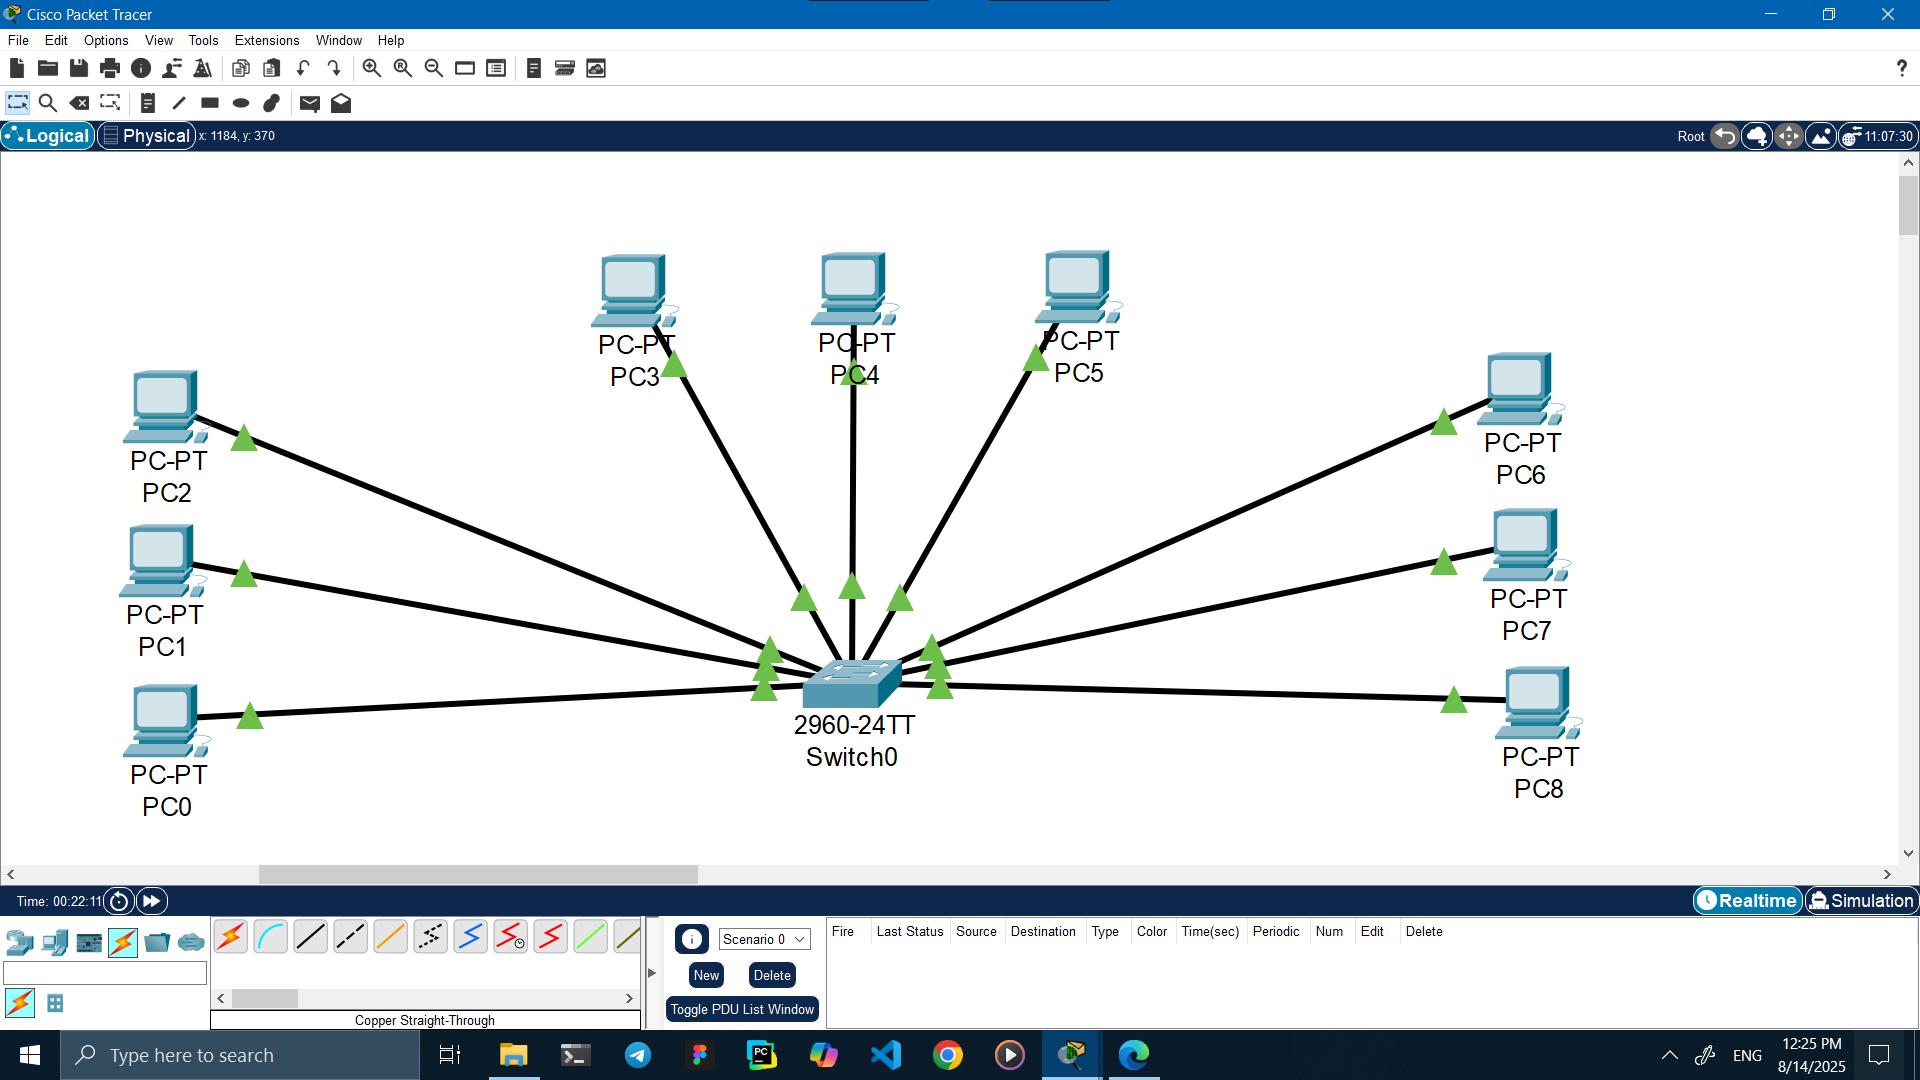
\includegraphics[width=\textwidth]{resources/1.png}
		\caption{ساخت سناریو  و اتصالات اولیهٔ آن}
		\label{img:1}
	\end{figure}
	\begin{figure}[H]
		\centering
		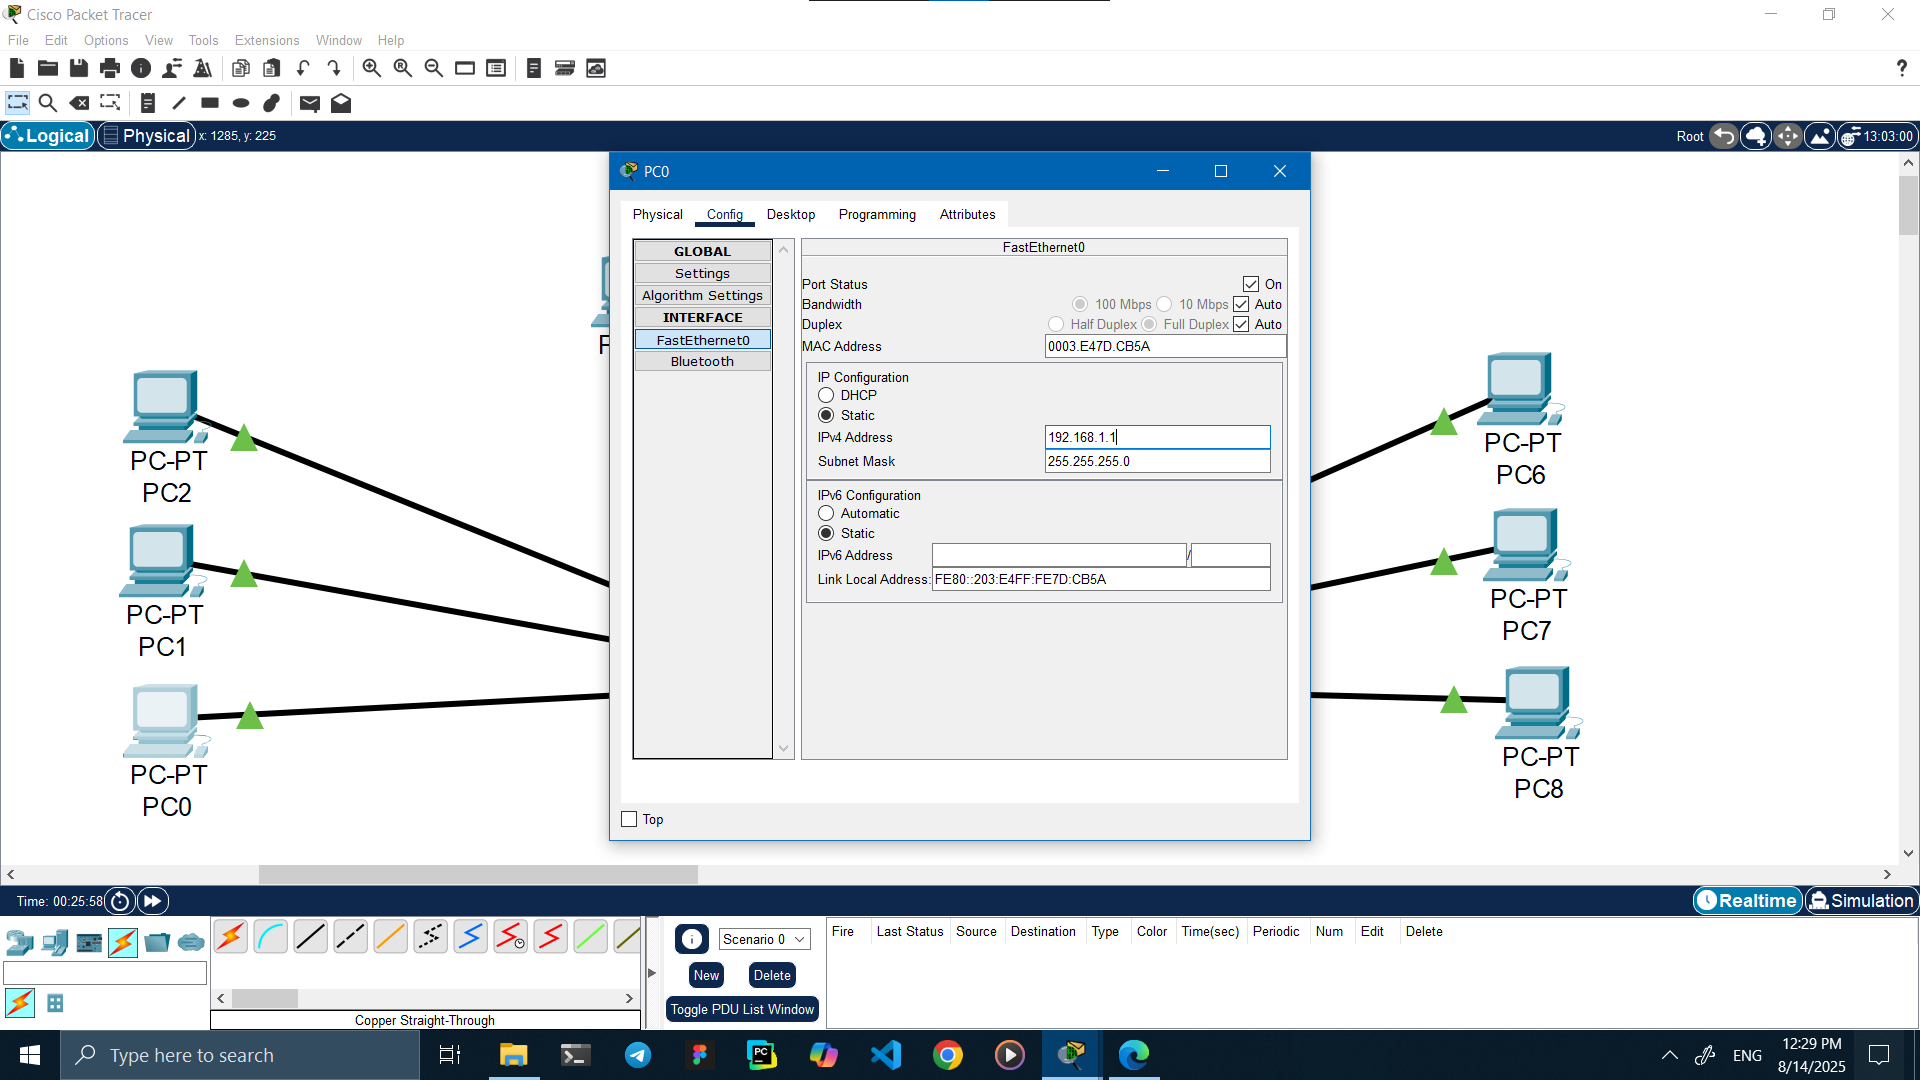
\includegraphics[width=\textwidth]{resources/2.png}
		\caption{تنظیم \textenglish{IP} برای \textenglish{PC0}}
		\label{img:2}
	\end{figure}
	\begin{figure}[H]
		\centering
		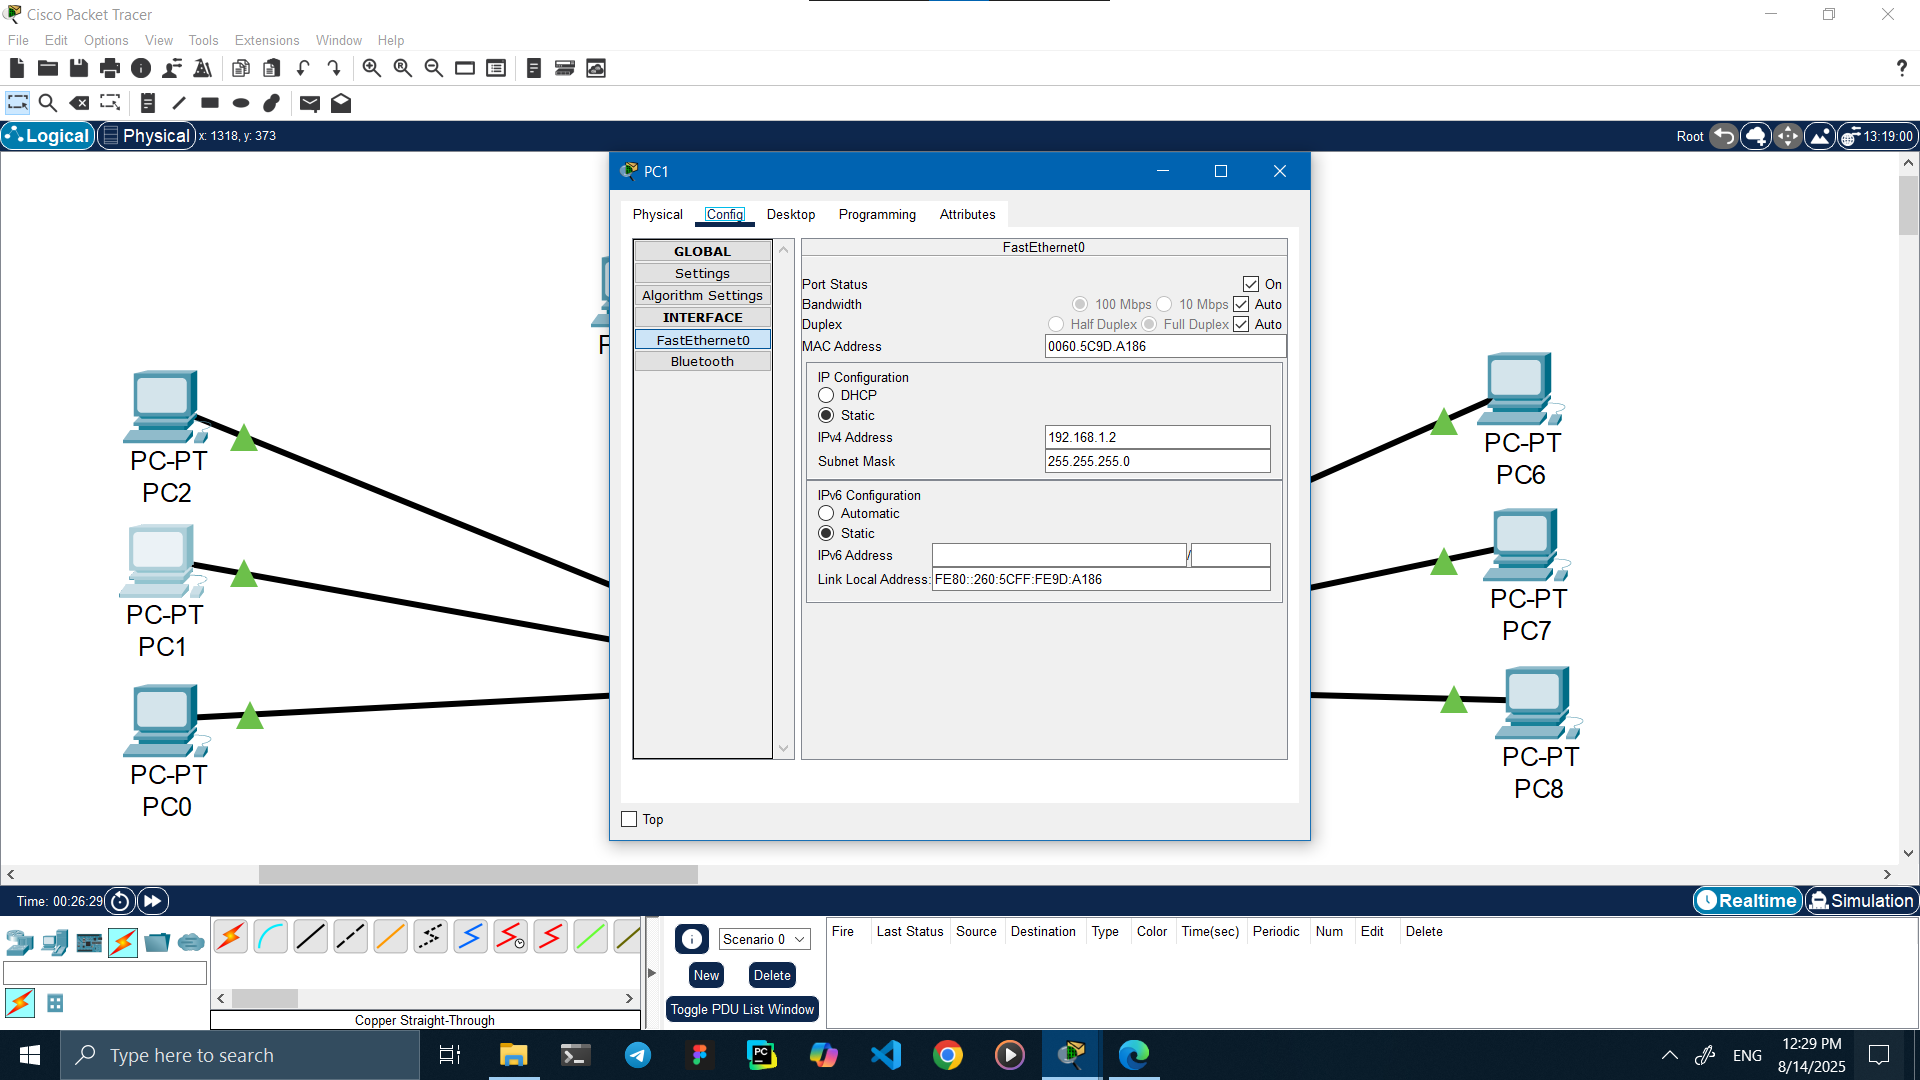
\includegraphics[width=\textwidth]{resources/2-1.png}
		\caption{تنظیم \textenglish{IP} برای \textenglish{PC1}}
		\label{img:2-1}
	\end{figure}
	\begin{figure}[H]
		\centering
		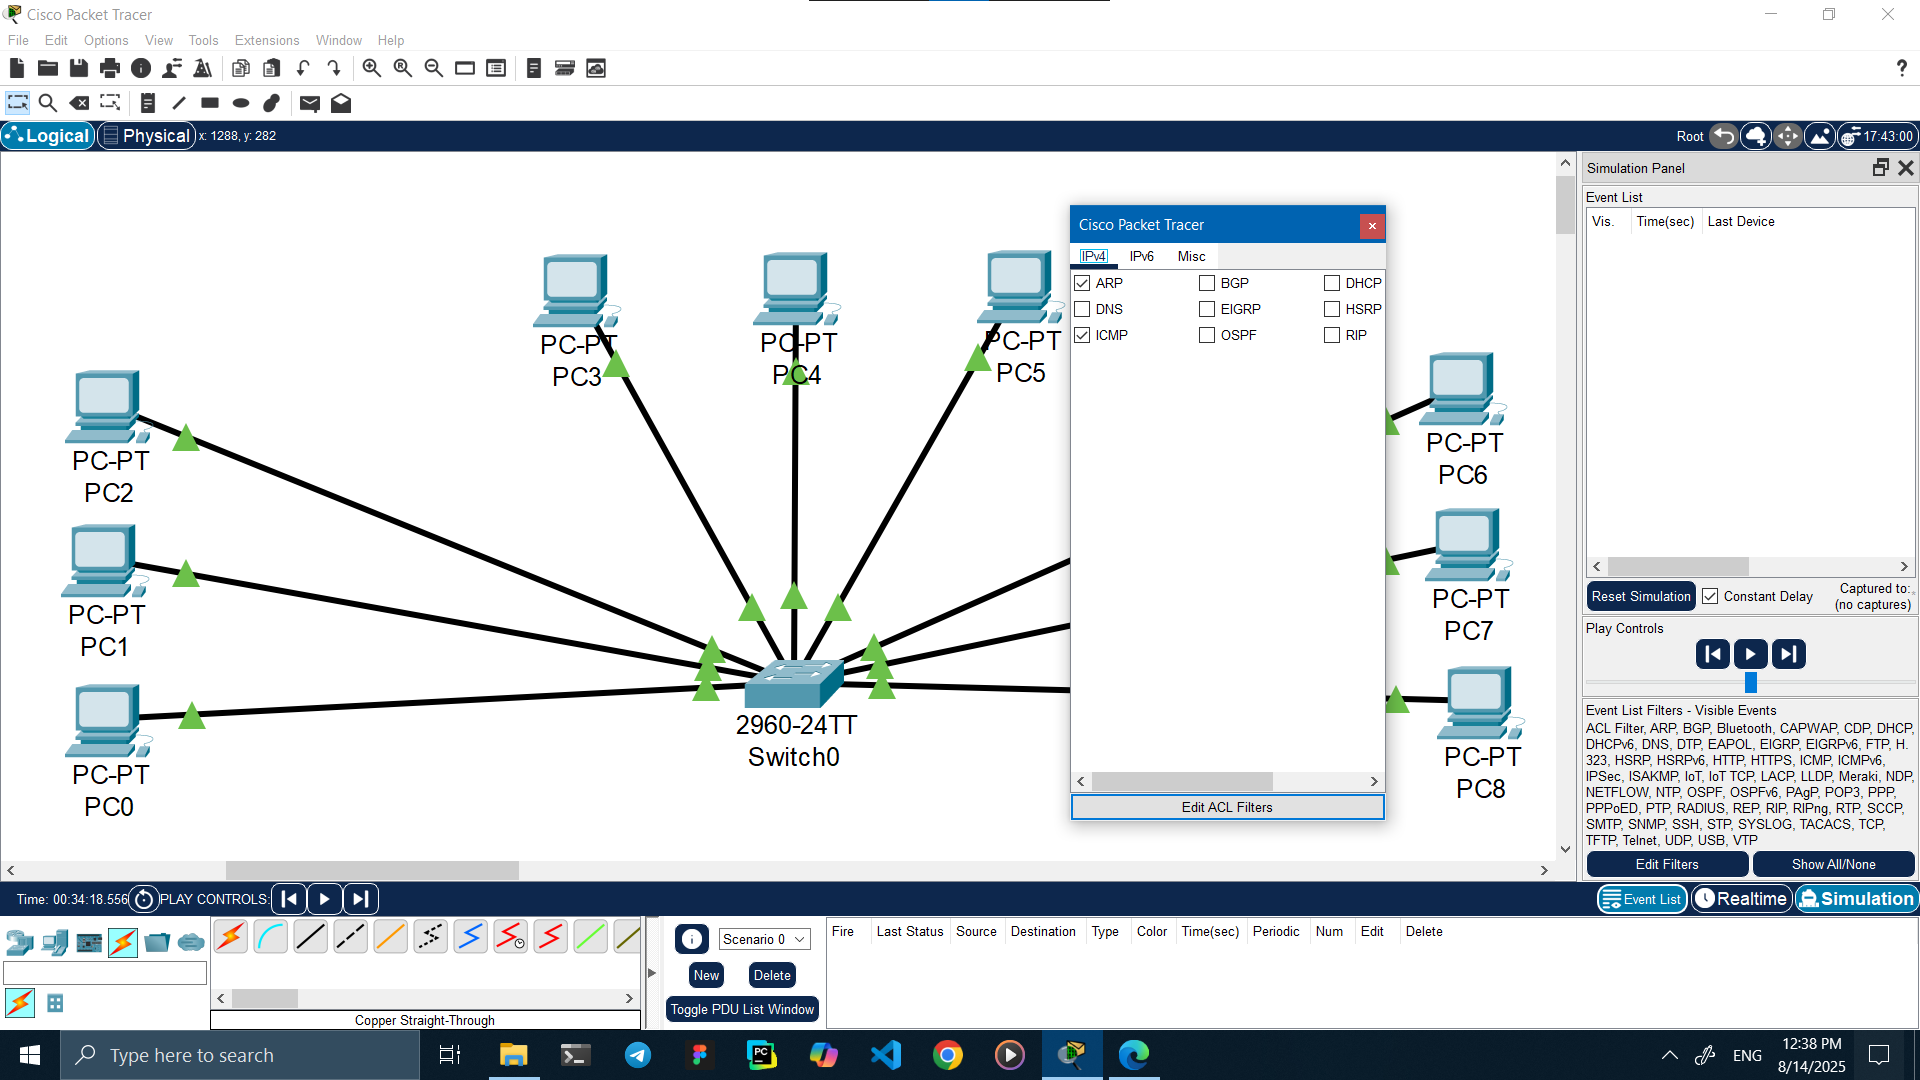
\includegraphics[width=\textwidth]{resources/3.png}
		\caption{فیلتر همه بسته‌ها به جز \textenglish{ARP} و \textenglish{ICMP}}
		\label{img:3}
	\end{figure}
	اکنون در بخش شبیه‌سازی، تنها بسته‌های \textenglish{ARP} و \textenglish{ICMP} را دنبال می‌کنیم. در ادامه از دستگاه \textenglish{PC0} دستور \textenglish{ping 192.168.1.2} را وارد می‌کنیم. شکل‌های \ref{img:4} و \ref{img:5} مراحل این شبیه‌سازی را نشان می‌دهند. همانطور که دیده می‌شود کل شبکه درگیر می‌شود. در شکل \ref{img:6} نیز نمایی از پرسش و پاسخ این دستور در دستگاه دیده می‌شود.
	\begin{figure}[H]
		\centering
		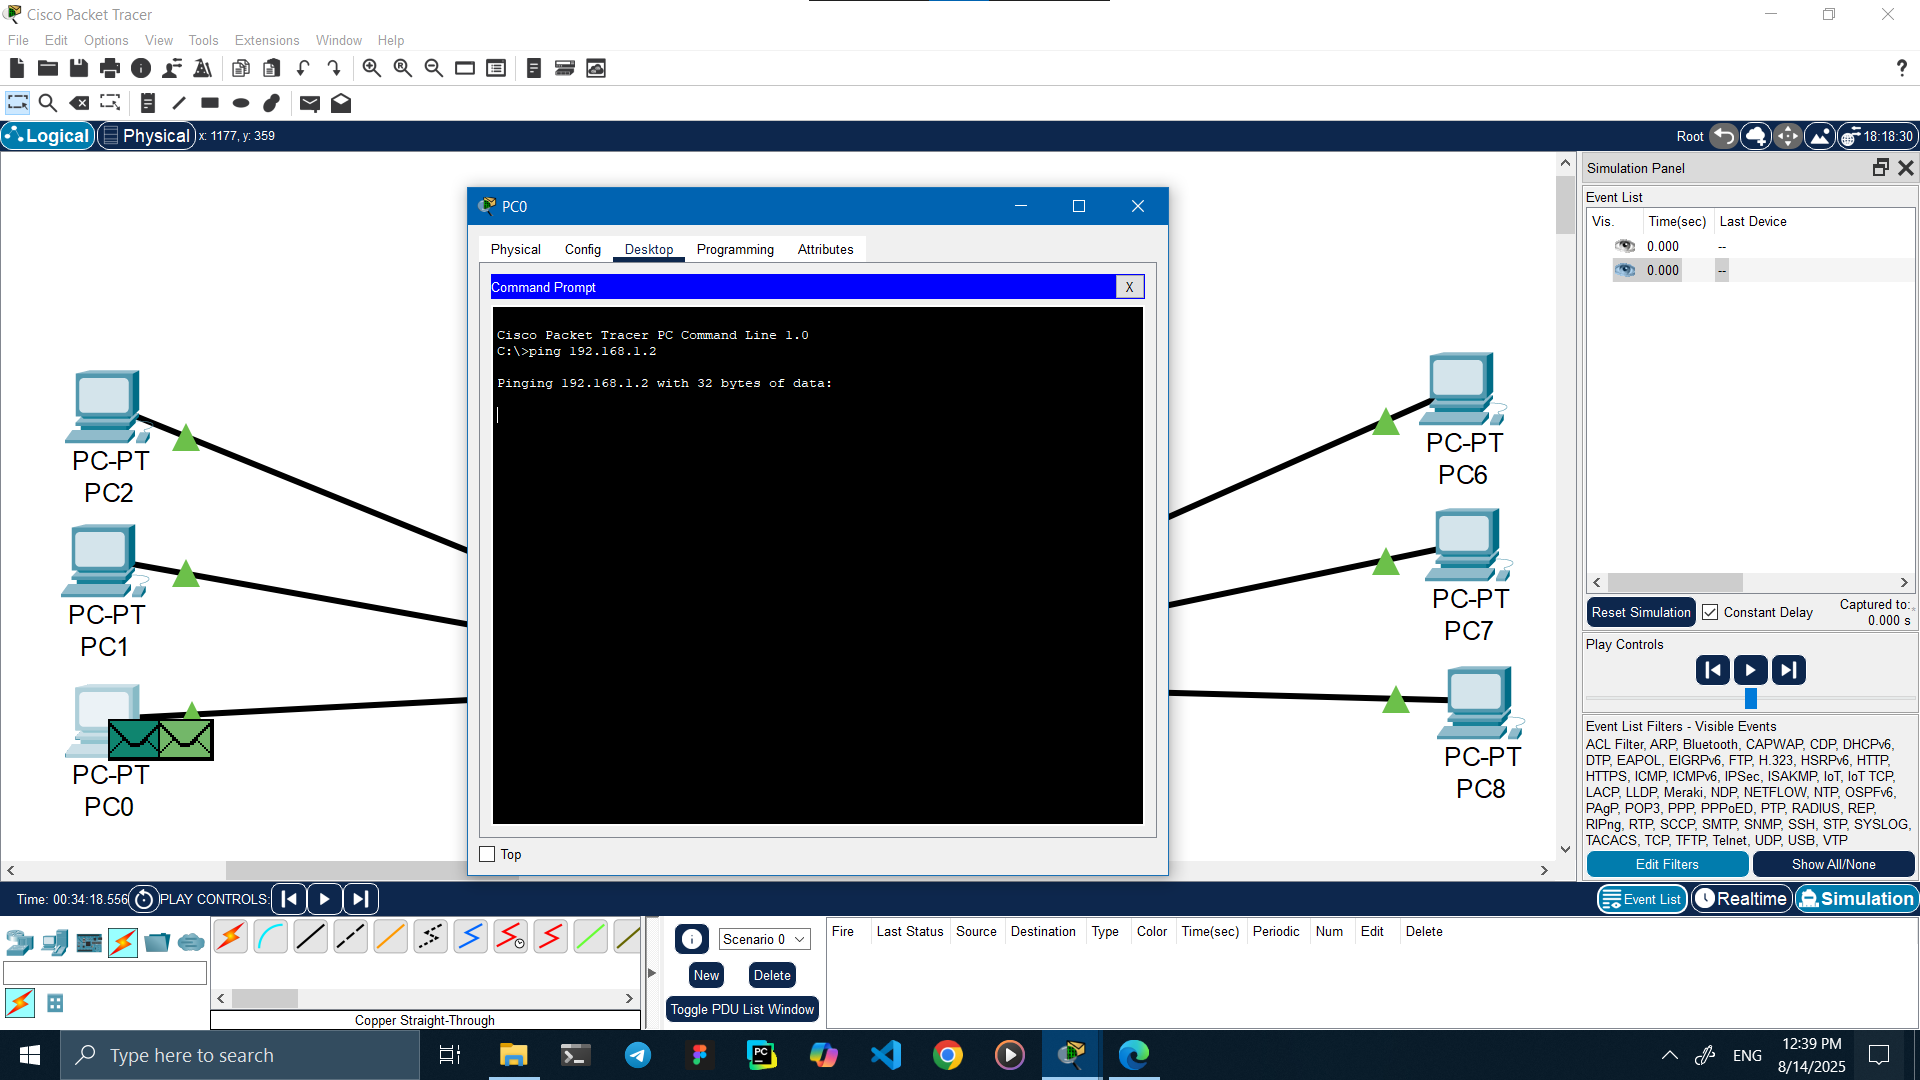
\includegraphics[width=\textwidth]{resources/4.png}
		\caption{ارسال بسته به تمام دستگاه‌‌های متصل در نتیجهٔ \textenglish{ping}}
		\label{img:4}
	\end{figure}
	\begin{figure}[H]
		\centering
		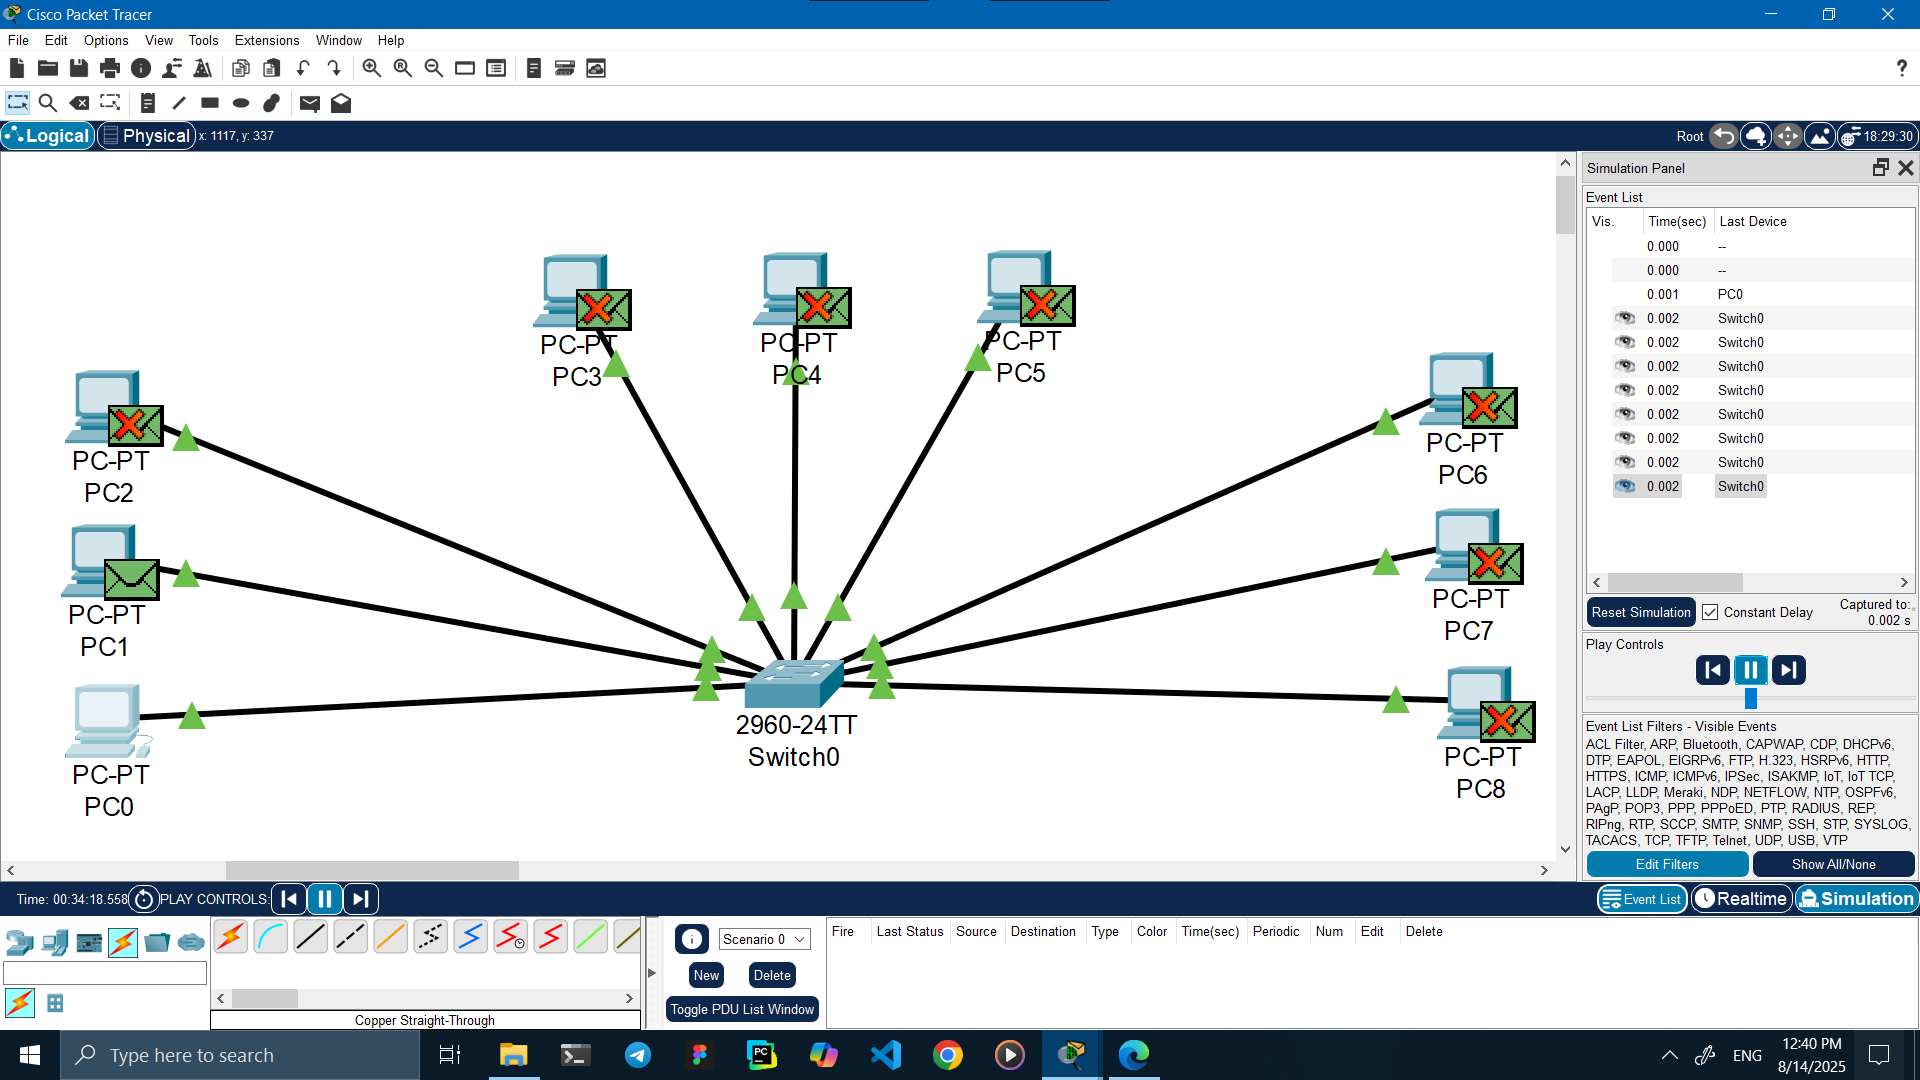
\includegraphics[width=\textwidth]{resources/5.png}
		\caption{بستهٔ \textenglish{ICMP} در حالت شبیه‌سازی}
		\label{img:5}
	\end{figure}
	\begin{figure}[H]
		\centering
		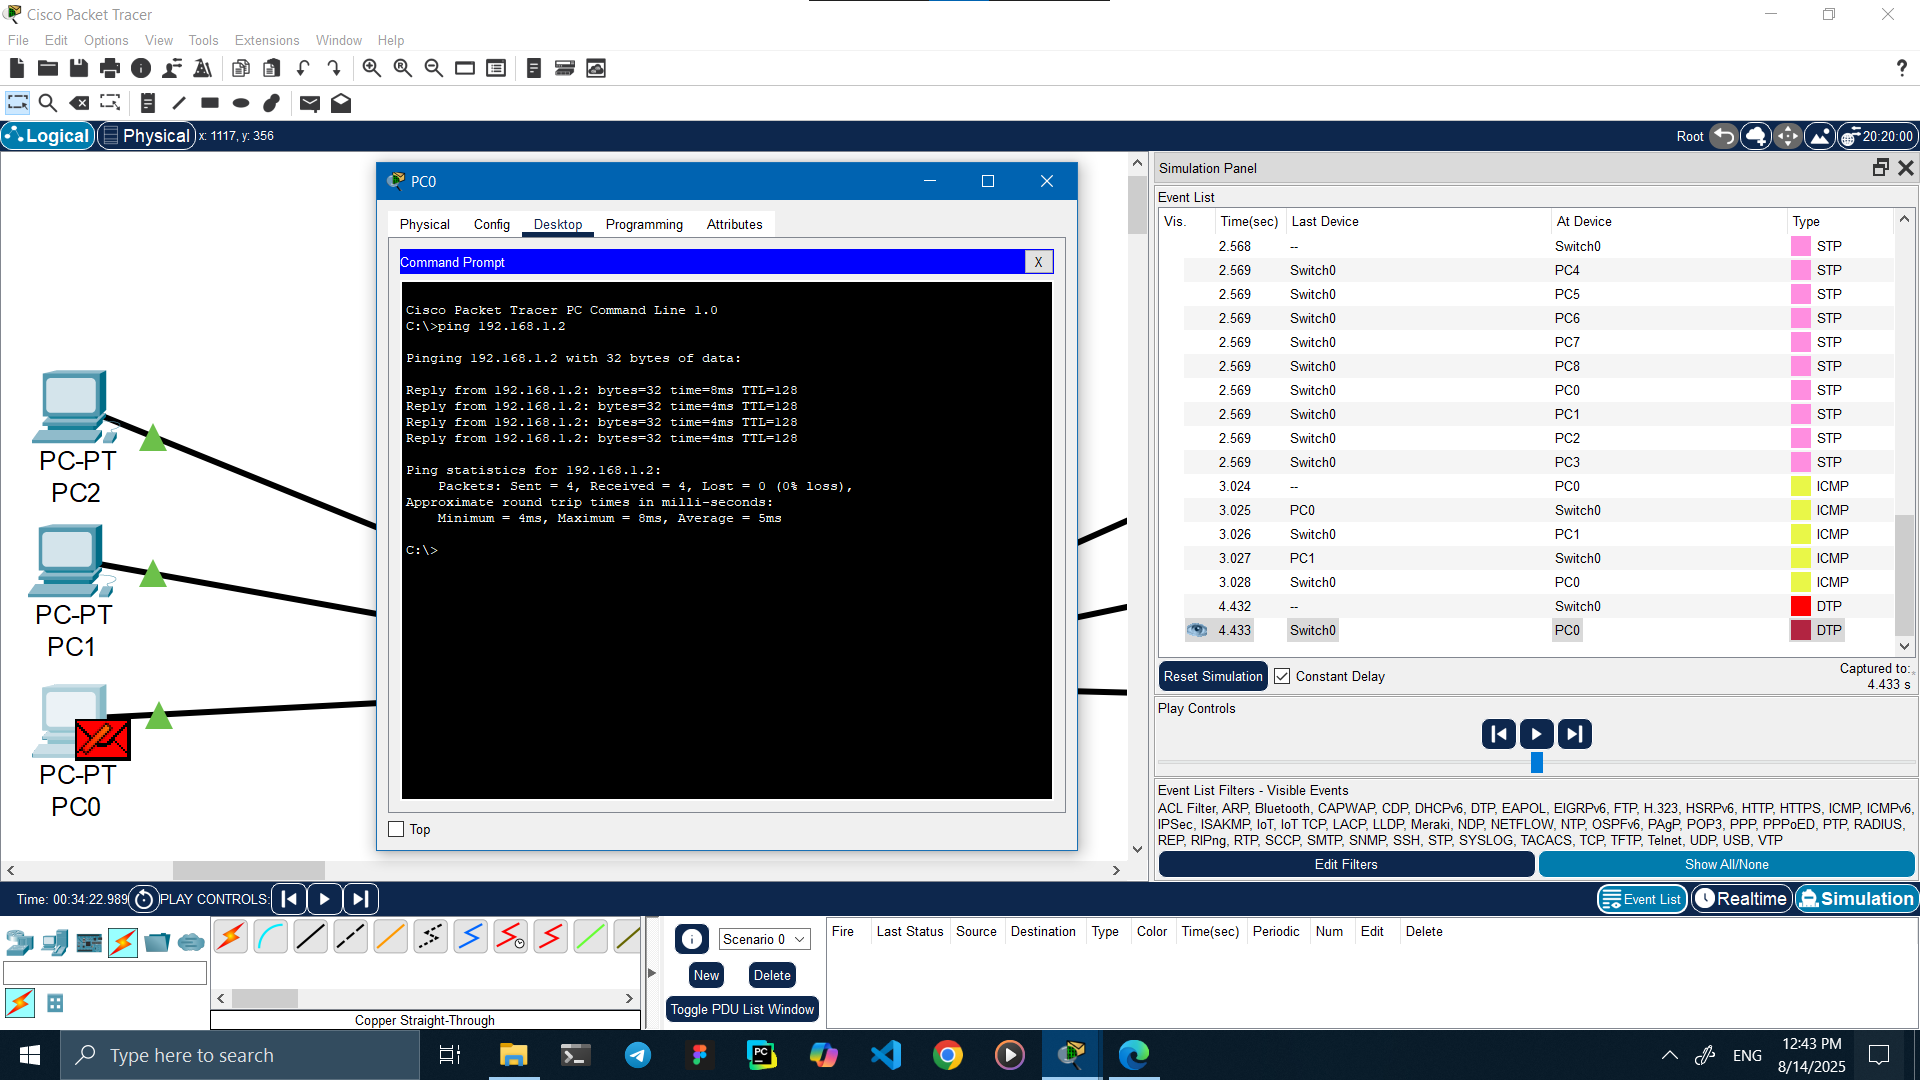
\includegraphics[width=\textwidth]{resources/6.png}
		\caption{نتیجهٔ دستور \textenglish{ping} در پایانهٔ دستگاه}
		\label{img:6}
	\end{figure}
	
	\newpage
	\section{سناریو ۲}
	در این سناریو، با همان چینش قبلی کار می‌کنیم. میخواهیم در سوییچ دستگاه‌ها را با ساخت \textenglish{VLAN} جدا کنیم. به \textenglish{VLAN} پیش‌فرض با شمارهٔ ۱ دو \textenglish{VLAN} جدید با نام‌های \textenglish{HR} و \textenglish{Sales} و شمارهٔ ۲ و ۳ می‌سازیم.به ترتیب شماره هر ۳ دستگاه در این \textenglish{VLAN} ها قرار می‌گیرند. دستگاه ۰ تا ۲ در شمارهٔ ۱، دستگاه ۳ تا ۵ در شمارهٔ ۳ و دستگاه ۶ تا ۸ در شمارهٔ ۳. در شکل \ref{img:7} انجام این فرآیند در سوییچ نشان داده شده است.
	\begin{figure}[H]
		\centering
		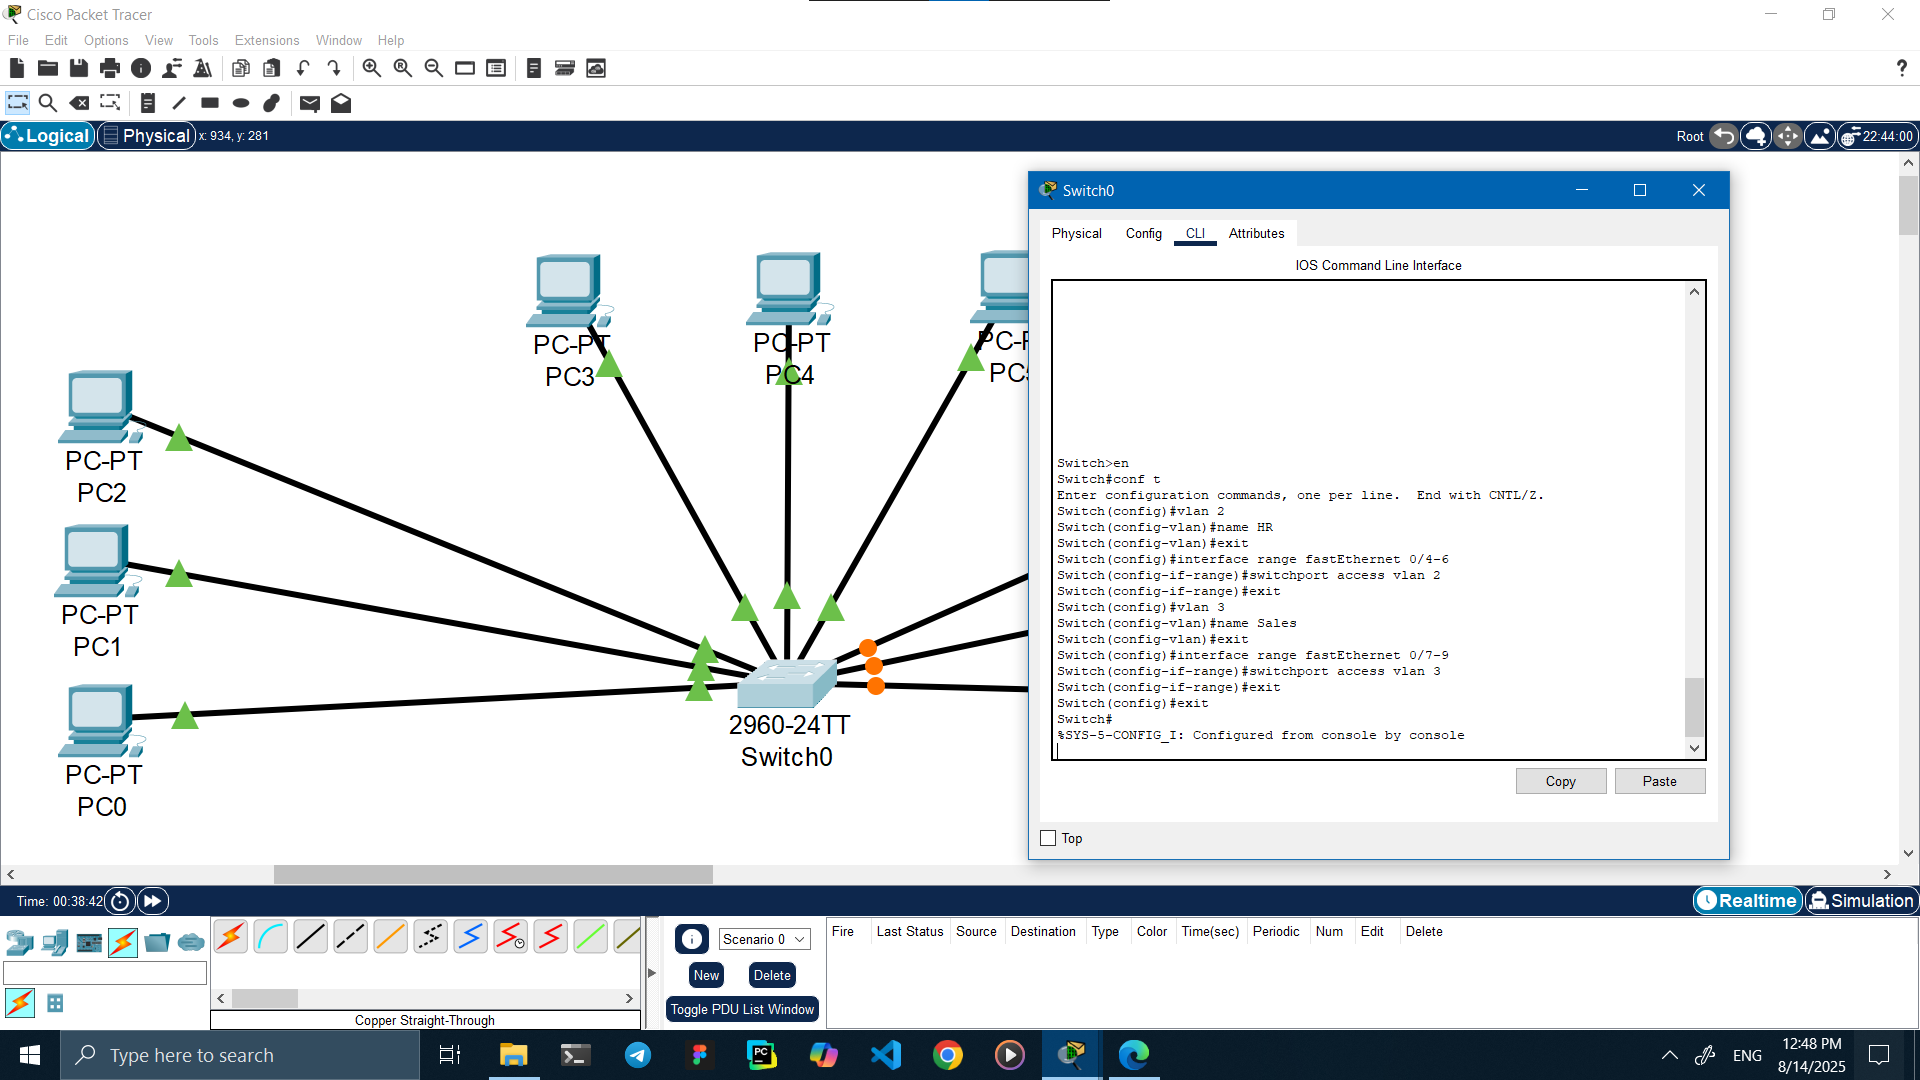
\includegraphics[width=\textwidth]{resources/7.png}
		\caption{اضافه کردن \textenglish{VLAN} ها در واسط سوییچ}
		\label{img:7}
	\end{figure}
	حال شکل \ref{img:8} وضعیت \textenglish{VLAN} ها و عضویت دستگاه‌ها در آن‌ها را نشان می‌دهد. اکنون مجدد همان دستور \textenglish{ping 192.168.1.2} را از دستگاه صفر اجرا می‌کنیم. شکل‌های \ref{img:9} و \ref{img:10} شبیه‌سازی حرکت بسته‌ها را نشان می‌دهد. در این حالت همانطور که انتظار داریم فقط \textenglish{VLAN} مربوطه درگیر می‌شود. نتیجه کار در دستگاه اجرا‌کننده دستور در شکل \ref{img:11} آمده است.
	\begin{figure}[H]
		\centering
		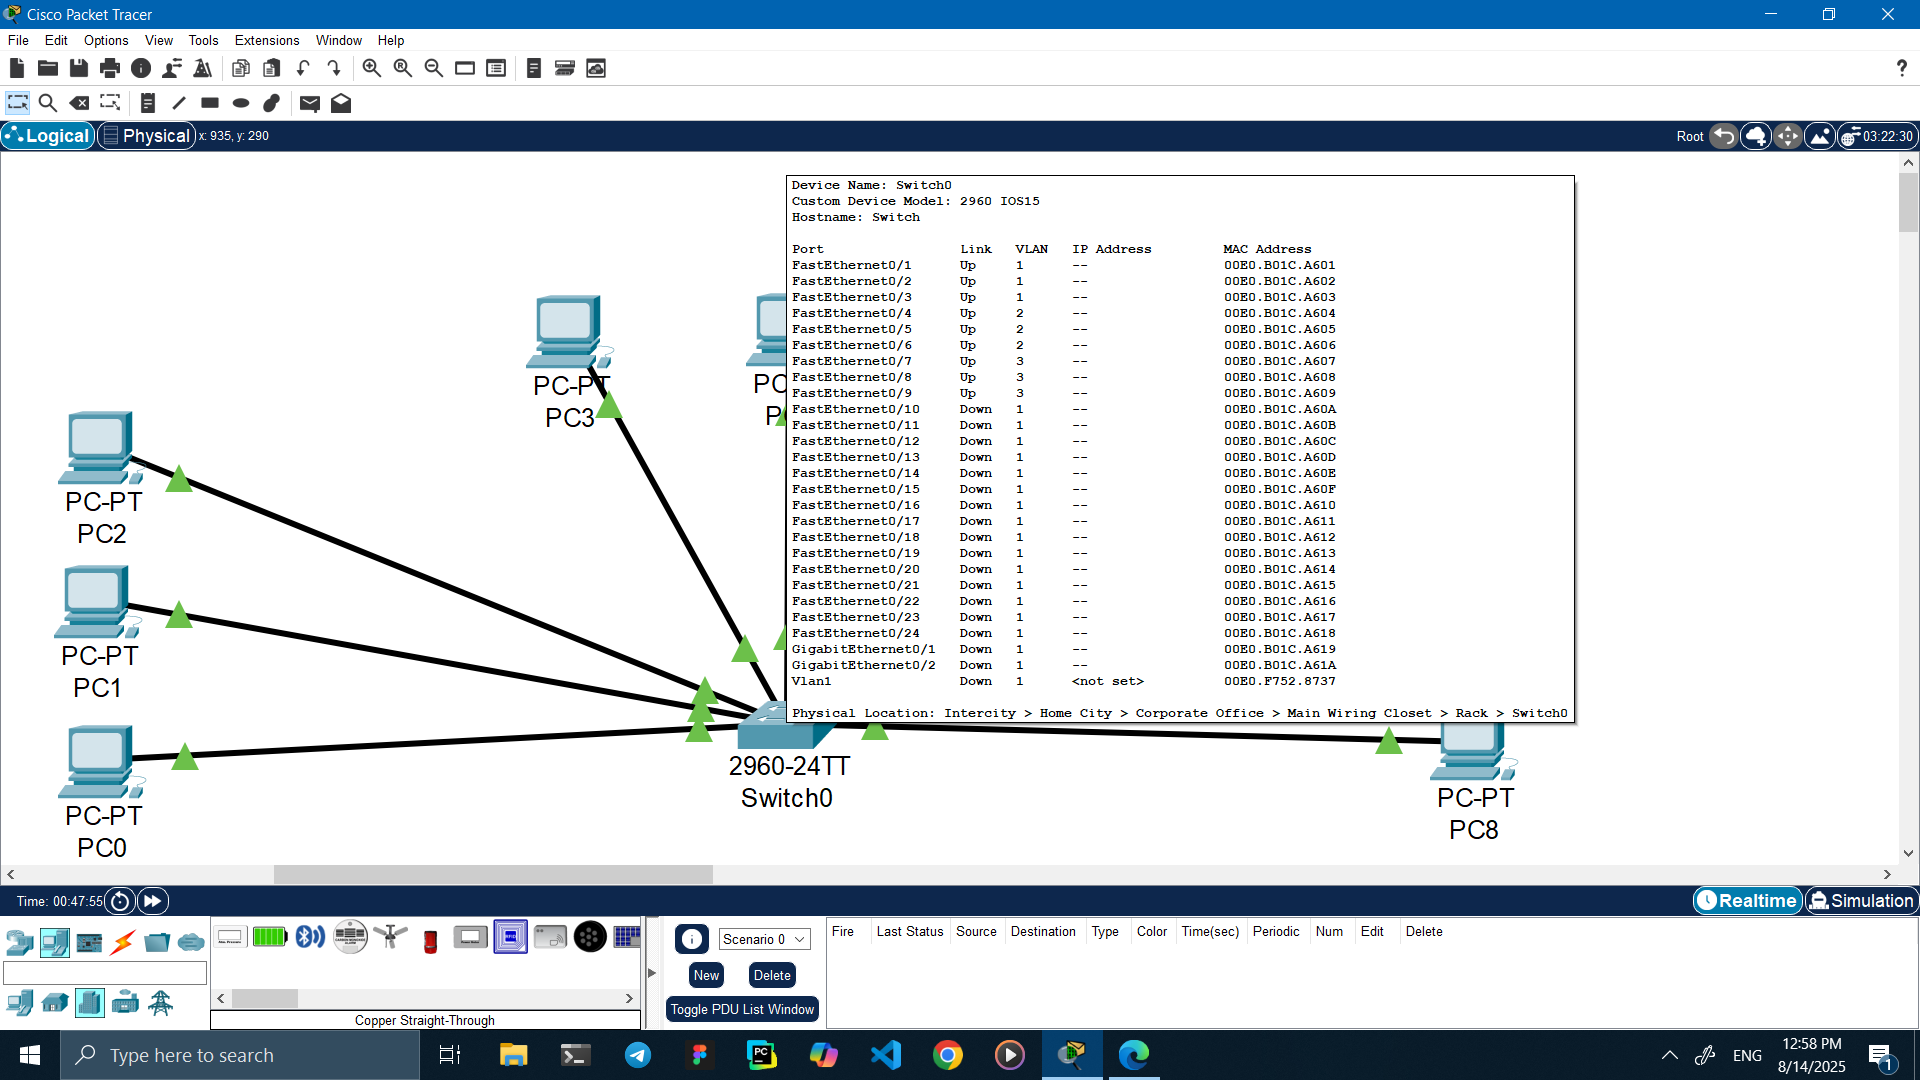
\includegraphics[width=\textwidth]{resources/8.png}
		\caption{وضعیت \textenglish{VLAN} ها در سوییچ و عضویت واسط‌ها در آنها}
		\label{img:8}
	\end{figure}
	\begin{figure}[H]
		\centering
		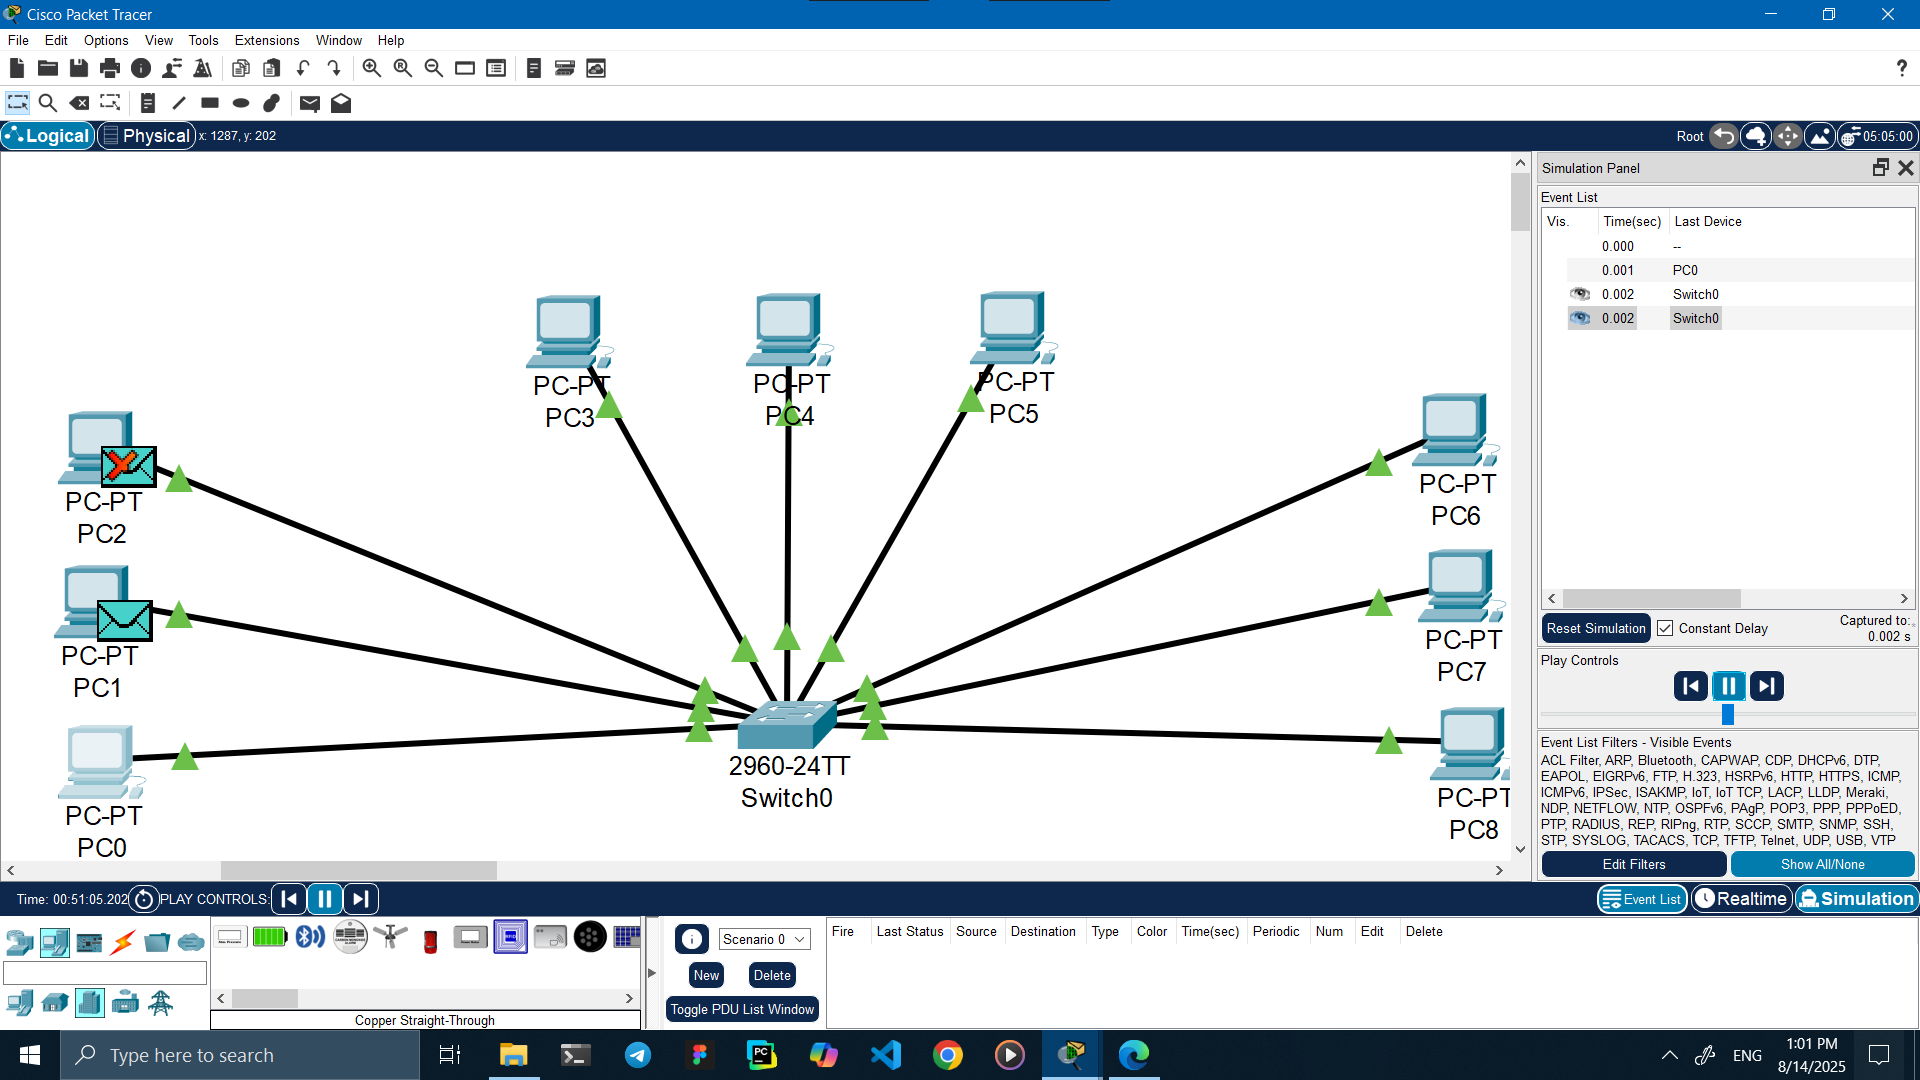
\includegraphics[width=\textwidth]{resources/9.png}
		\caption{ارسال بسته به فقط اعضای همان \textenglish{VLAN}}
		\label{img:9}
	\end{figure}
	\begin{figure}[H]
		\centering
		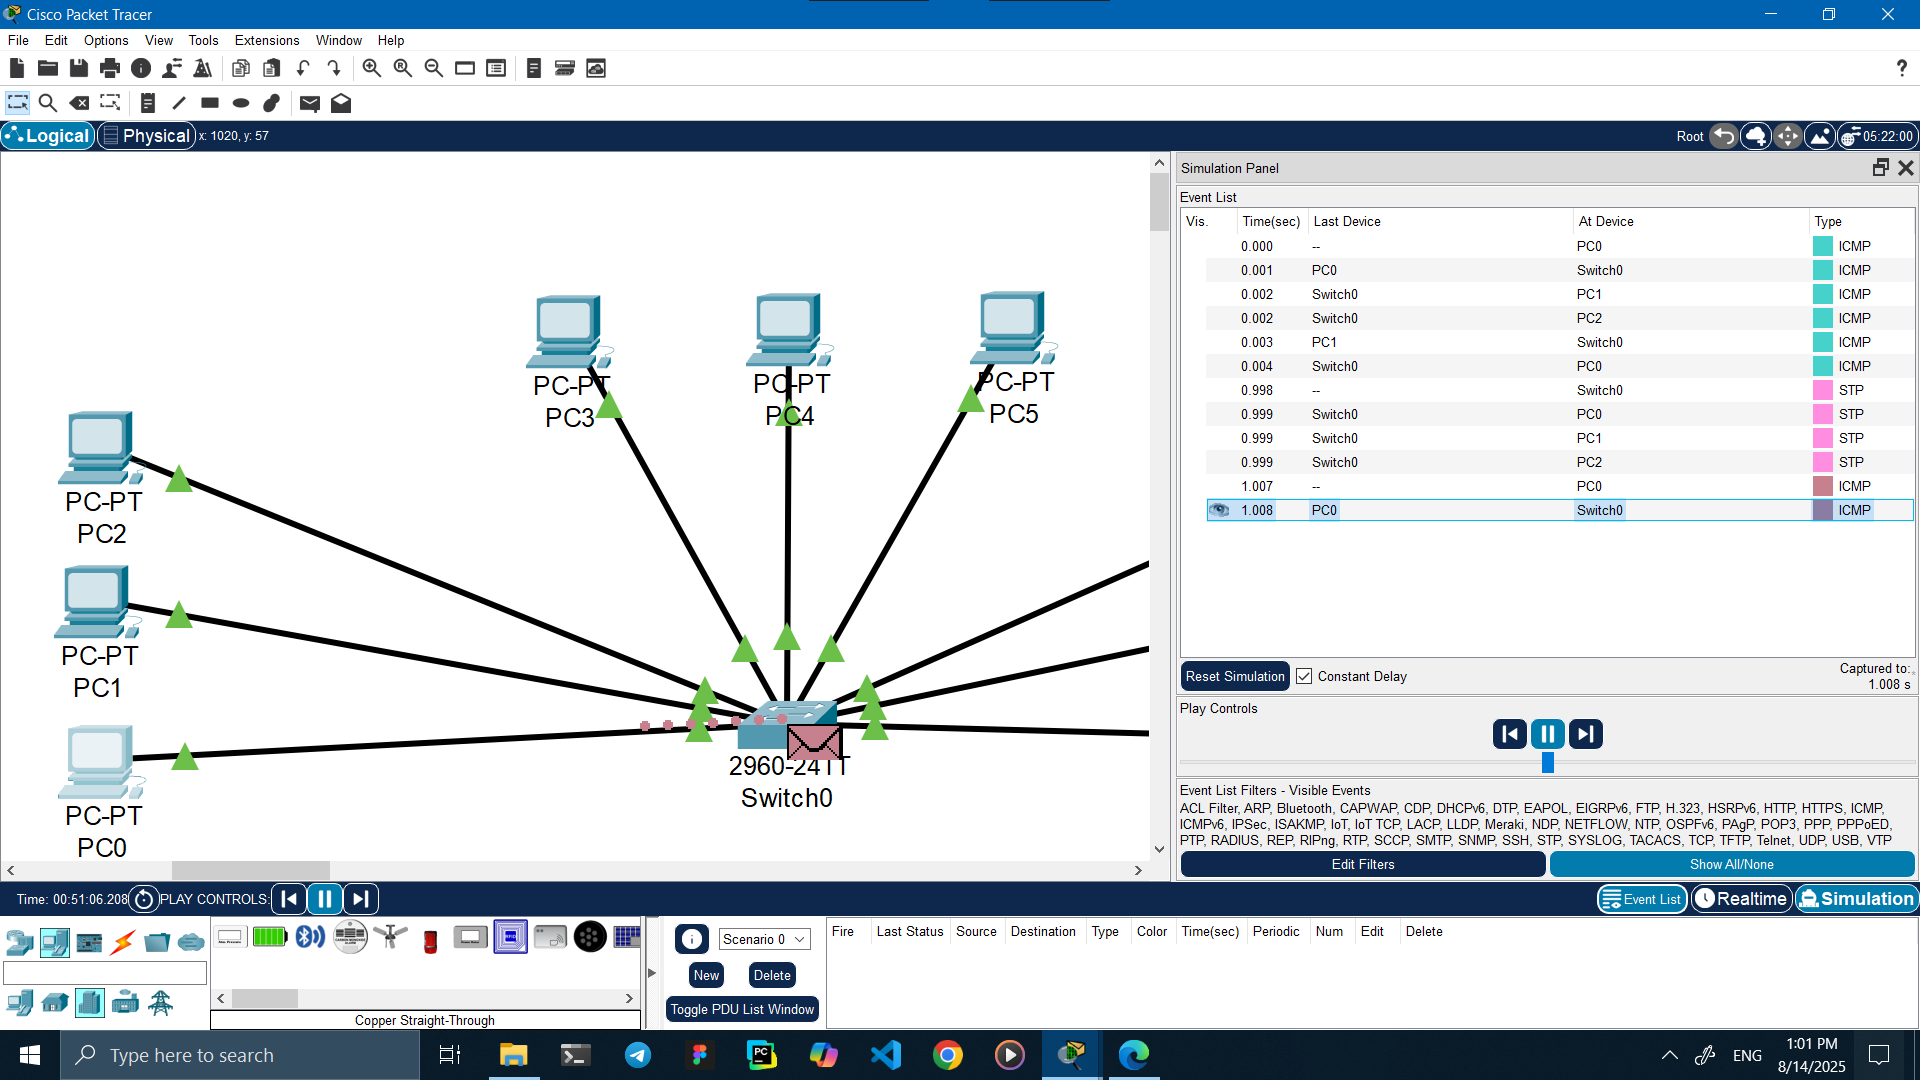
\includegraphics[width=\textwidth]{resources/10.png}
		\caption{حرکت بستهٔ \textenglish{ICMP}}
		\label{img:10}
	\end{figure}
	\begin{figure}[H]
		\centering
		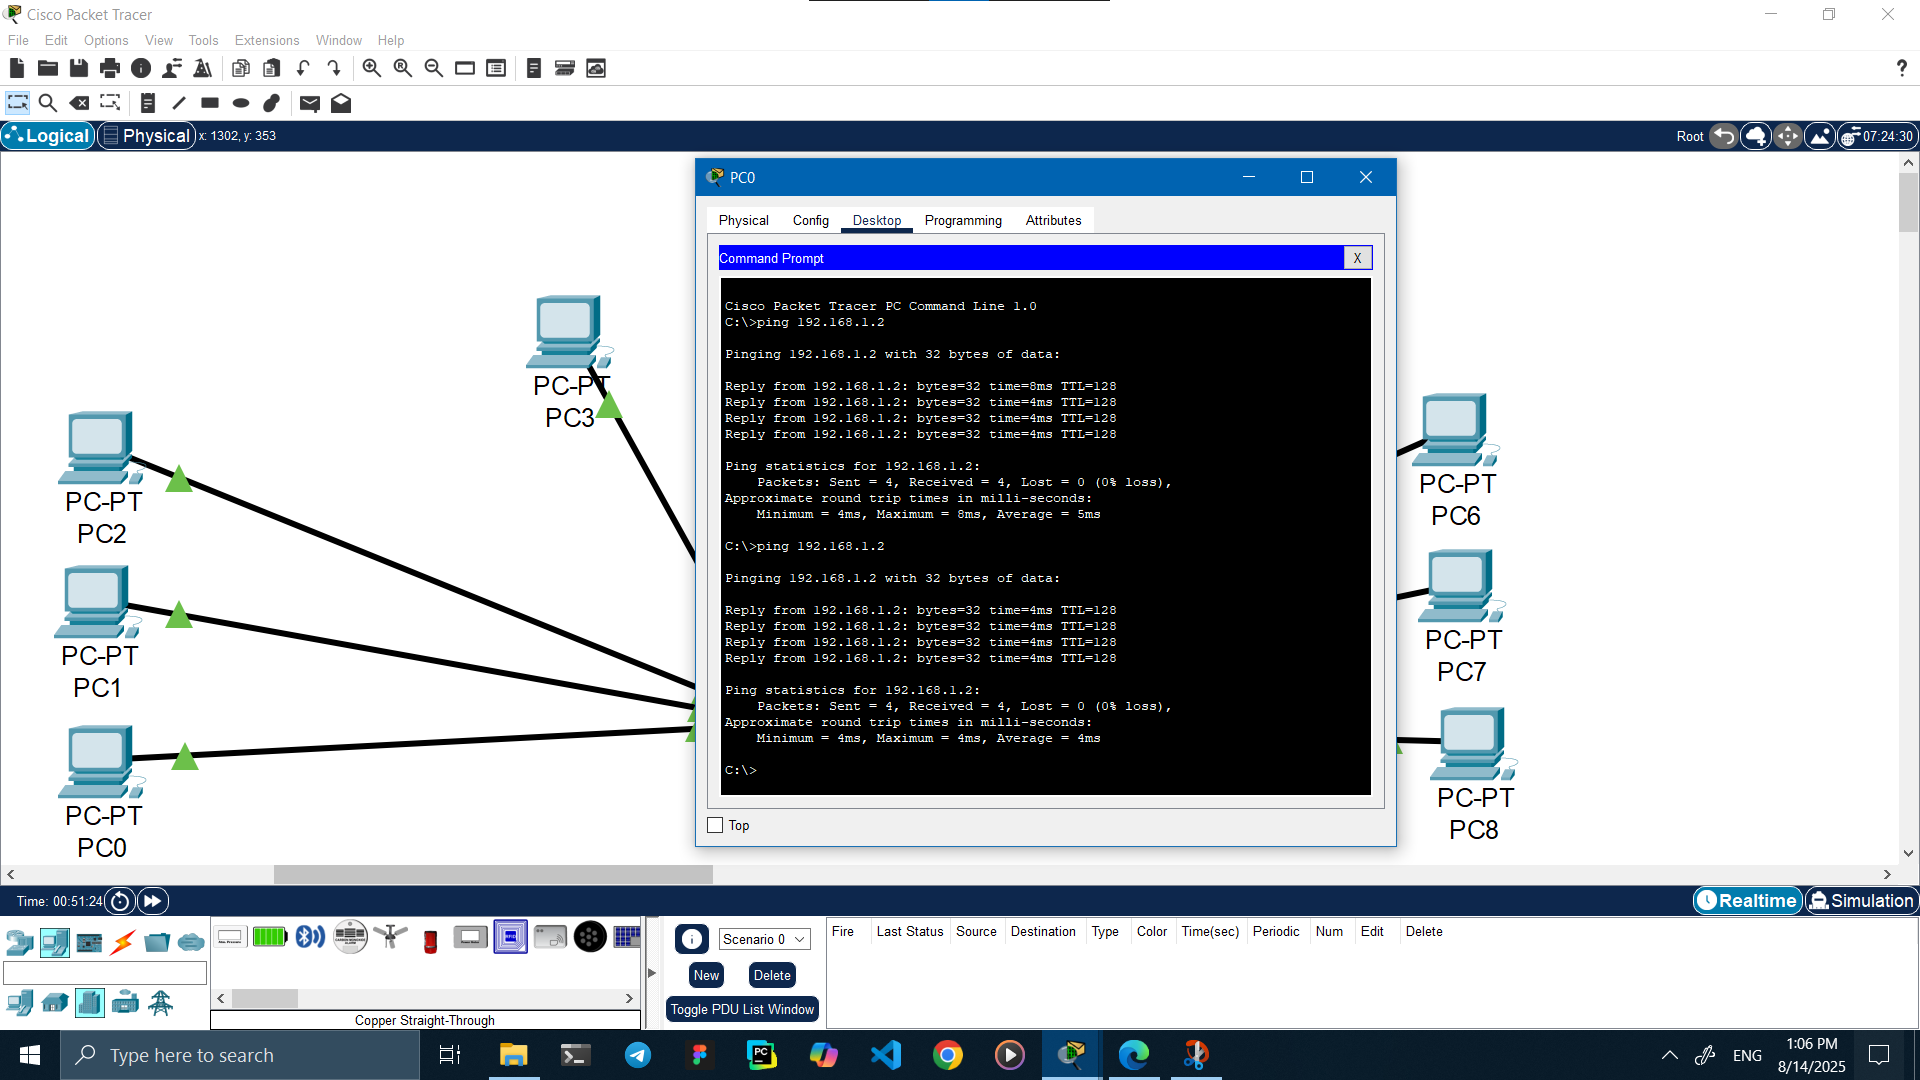
\includegraphics[width=\textwidth]{resources/11.png}
		\caption{نتیجهٔ دستور \textenglish{ping} در حالت جدید}
		\label{img:11}
	\end{figure}
	
	\newpage
	\section{سناریو ۳}
	در این سناریو یک چیدمان از ۳ زیرشبکهٔ متفاوت ولی متصل با سوییچ با فضای آدرس نشان داده شده در شکل \ref{img:12} درست می‌کنیم. در اینجا همان \textenglish{VLAN} های قبلی را داریم و هر زیرشبکه به ترتیب شماره‌اش به یک \textenglish{VLAN} متناظر می‌شود. نمونهٔ تخصیص آدرس در شکل \ref{img:13} نشان داده شده است. مشابه سناریو قبل برای ایجاد و عملیاتی کردن \textenglish{VLAN} ها مانند شکل \ref{img:14} جلو می‌رویم. برای دیدن نتیجهٔ کار دستور \textenglish{show vlan} را در سوییچ اجرا می‌کنیم. نتیجه مانند شکل \ref{img:15} است. همچنین نتیجه دستور \textenglish{show vlan brief} نیز در شکل \ref{img:16} آمده است.
	\begin{figure}[H]
		\centering
		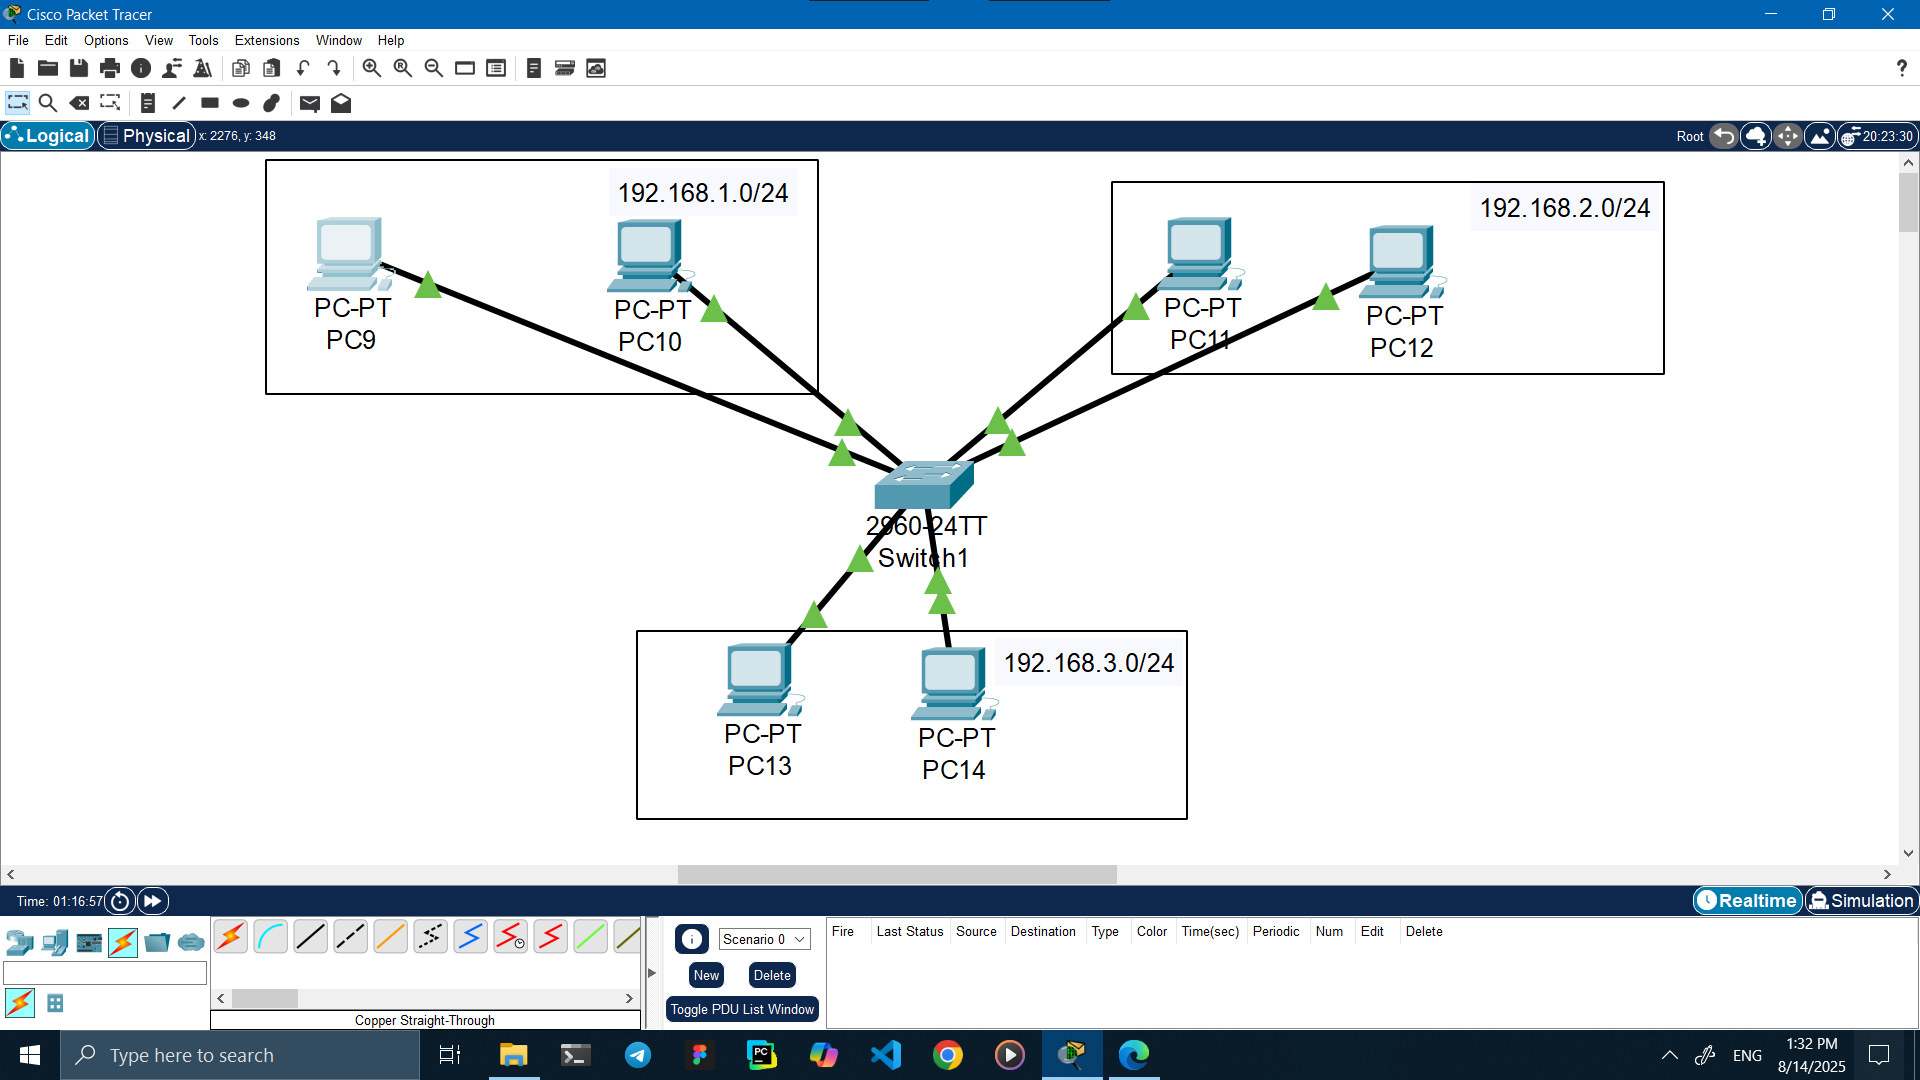
\includegraphics[width=\textwidth]{resources/12.png}
		\caption{طراحی سناریو جدید با ۳ زیرشبکه متصل به سوییچ}
		\label{img:12}
	\end{figure}
	\begin{figure}[H]
		\centering
		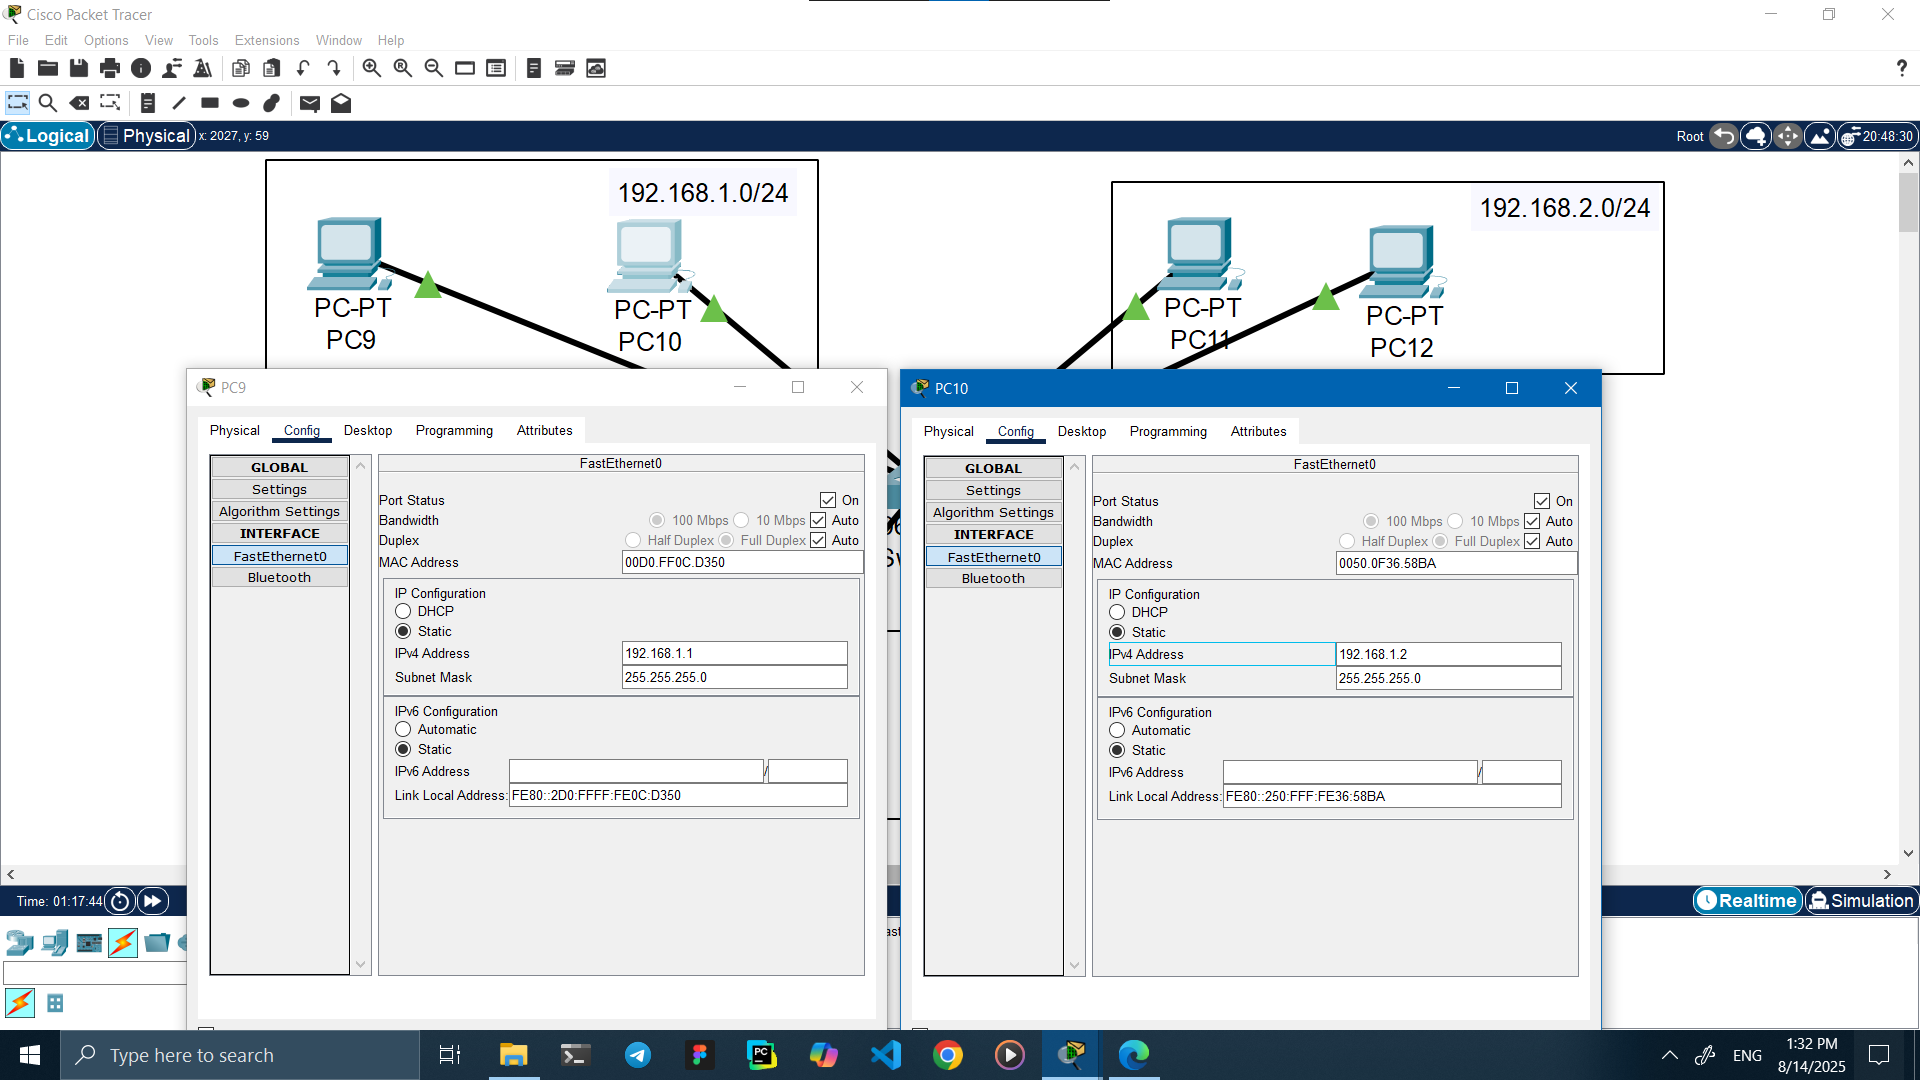
\includegraphics[width=\textwidth]{resources/13.png}
		\caption{تنظیم \textenglish{IP} برای اولین دستگاه این سناریو}
		\label{img:13}
	\end{figure}
	\begin{figure}[H]
		\centering
		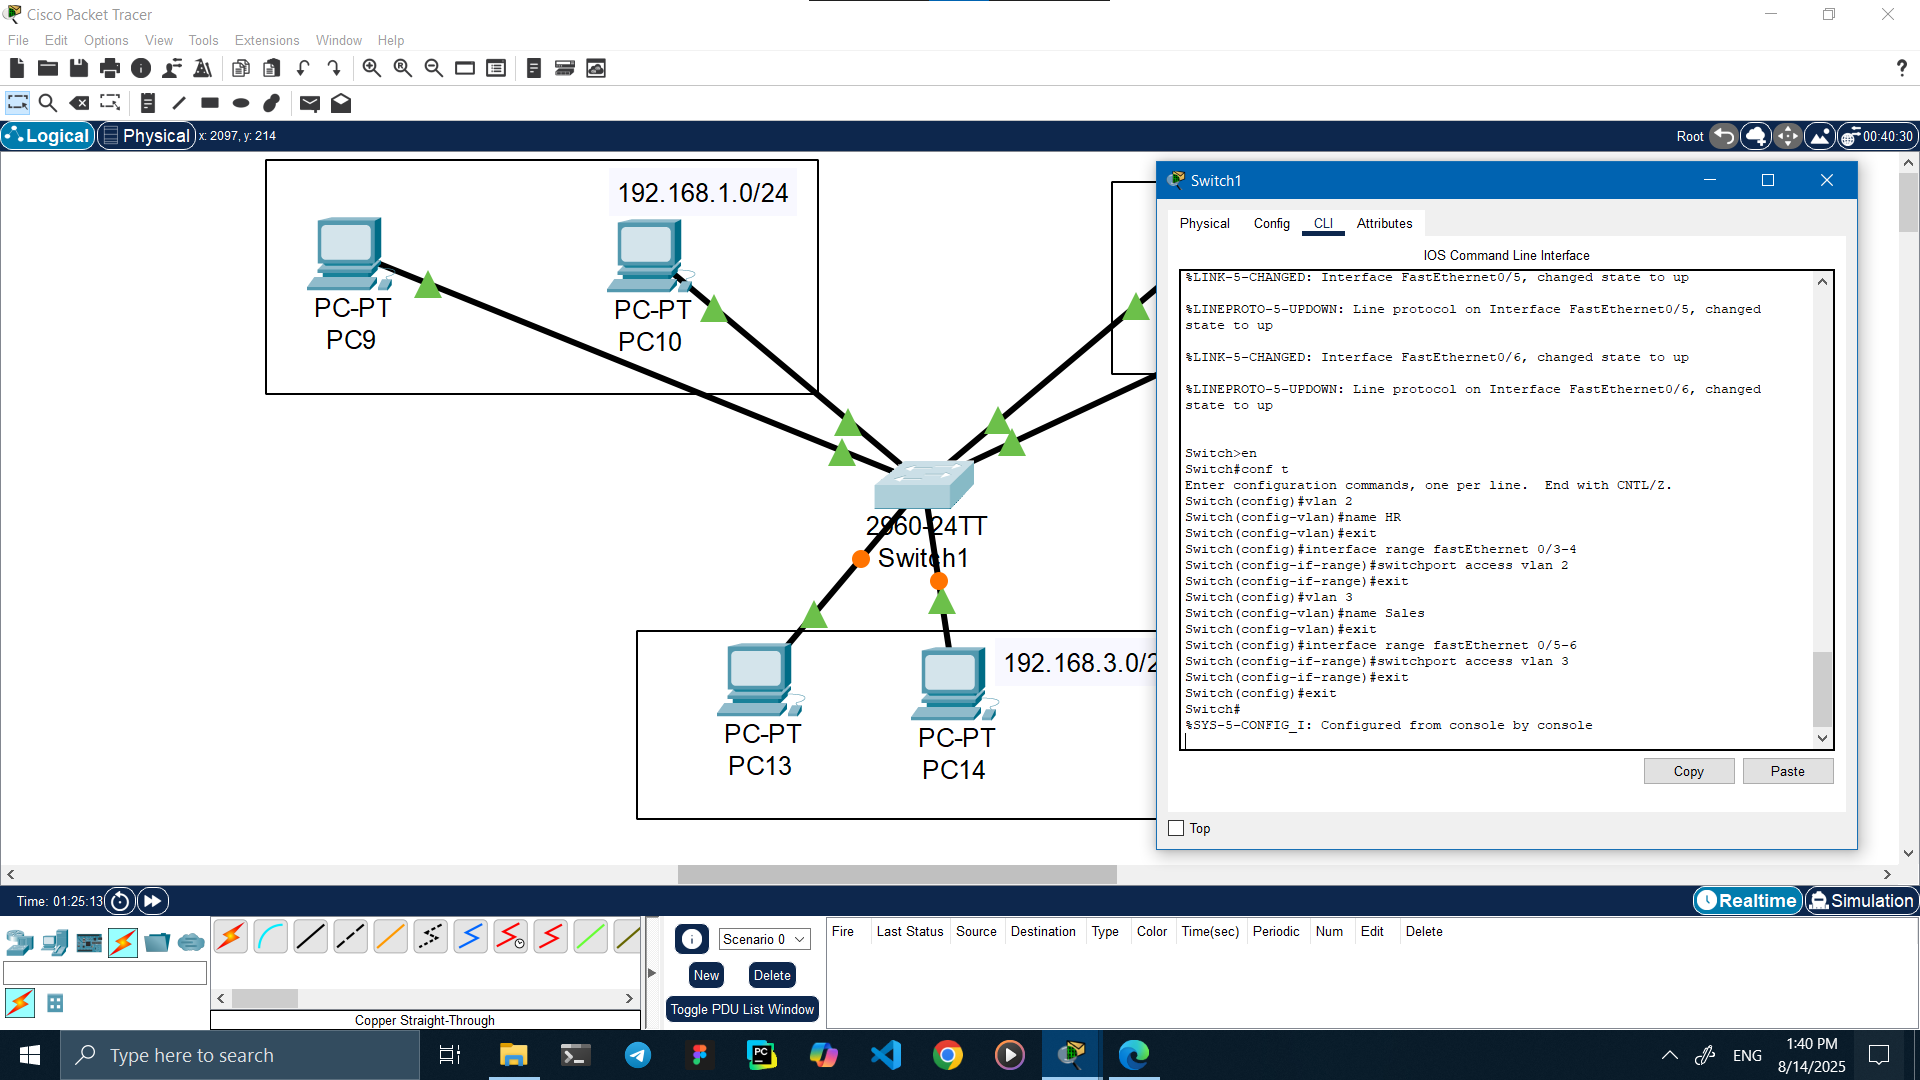
\includegraphics[width=\textwidth]{resources/14.png}
		\caption{اضافه کردن \textenglish{VLAN} ها در سوییچ}
		\label{img:14}
	\end{figure}
	\begin{figure}[H]
		\centering
		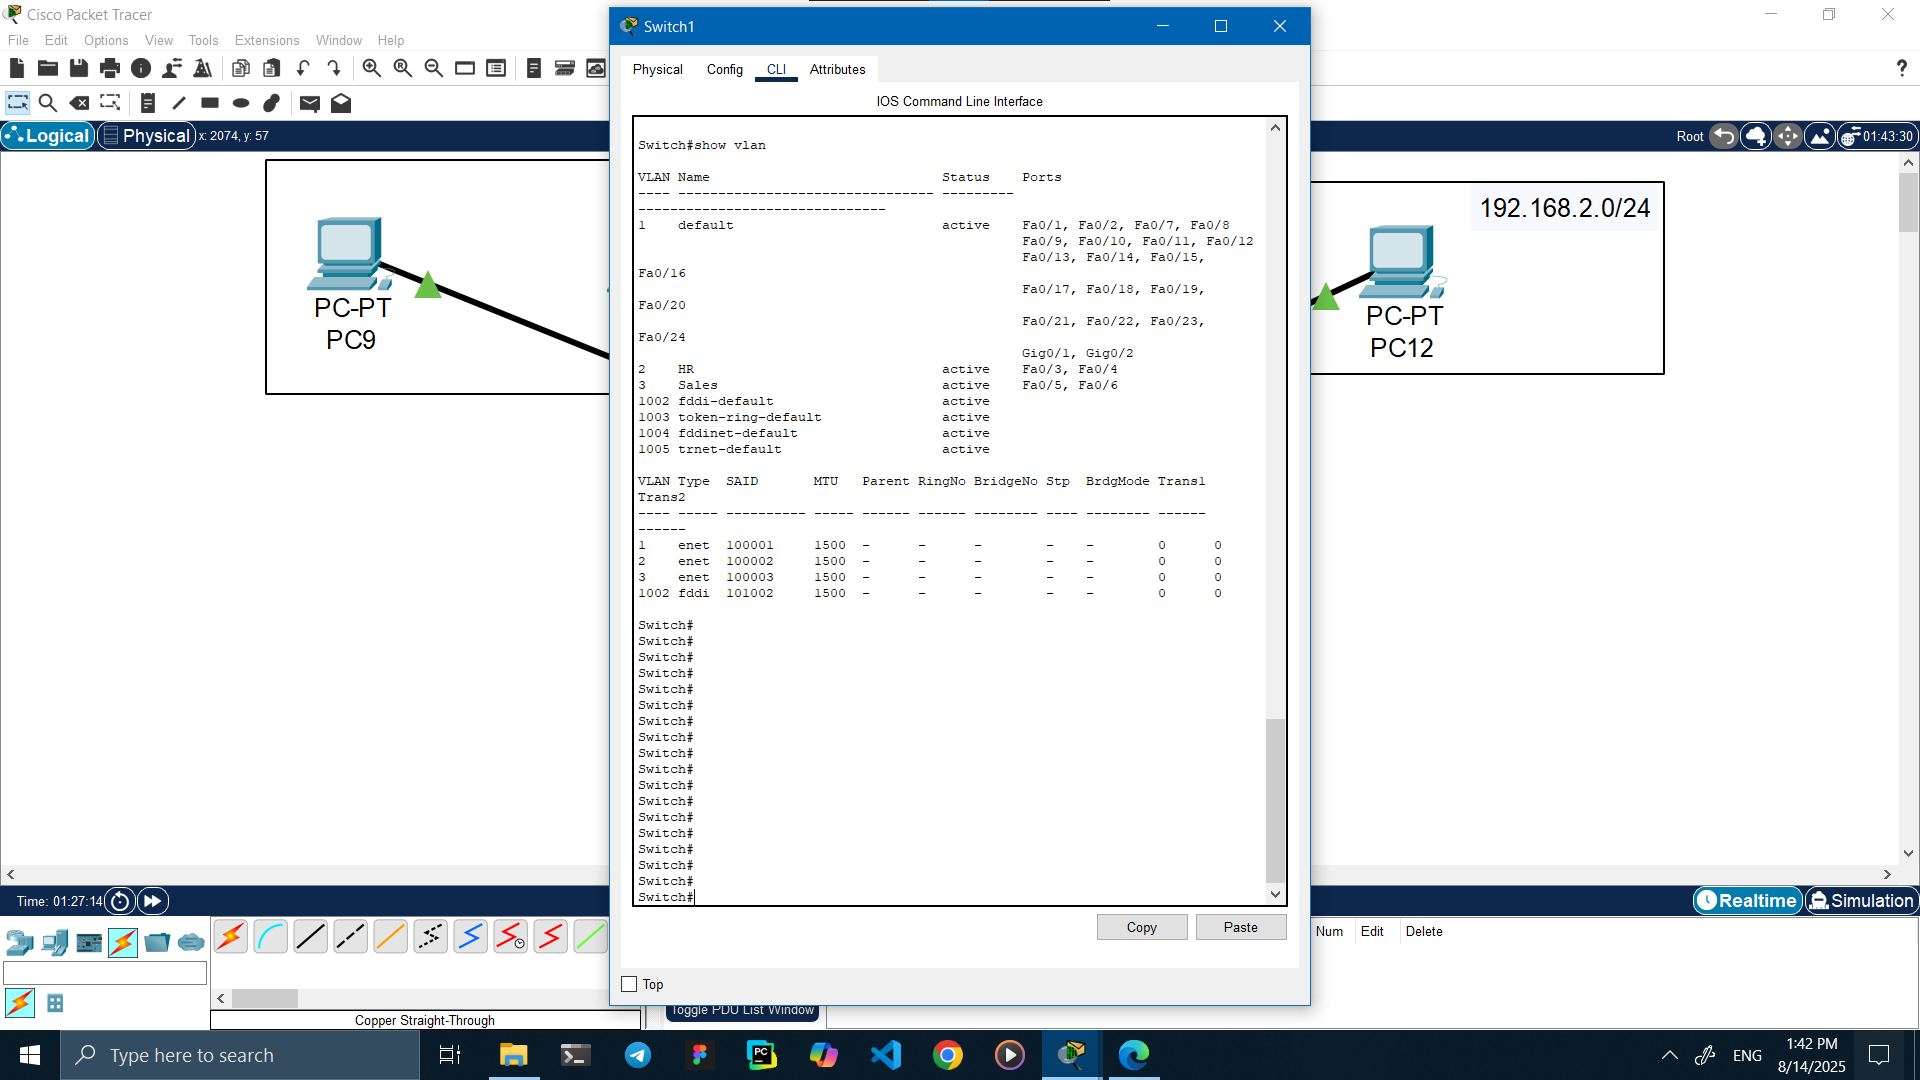
\includegraphics[width=\textwidth]{resources/15.png}
		\caption{اجرای دستور \textenglish{show vlan}}
		\label{img:15}
	\end{figure}
	\begin{figure}[H]
		\centering
		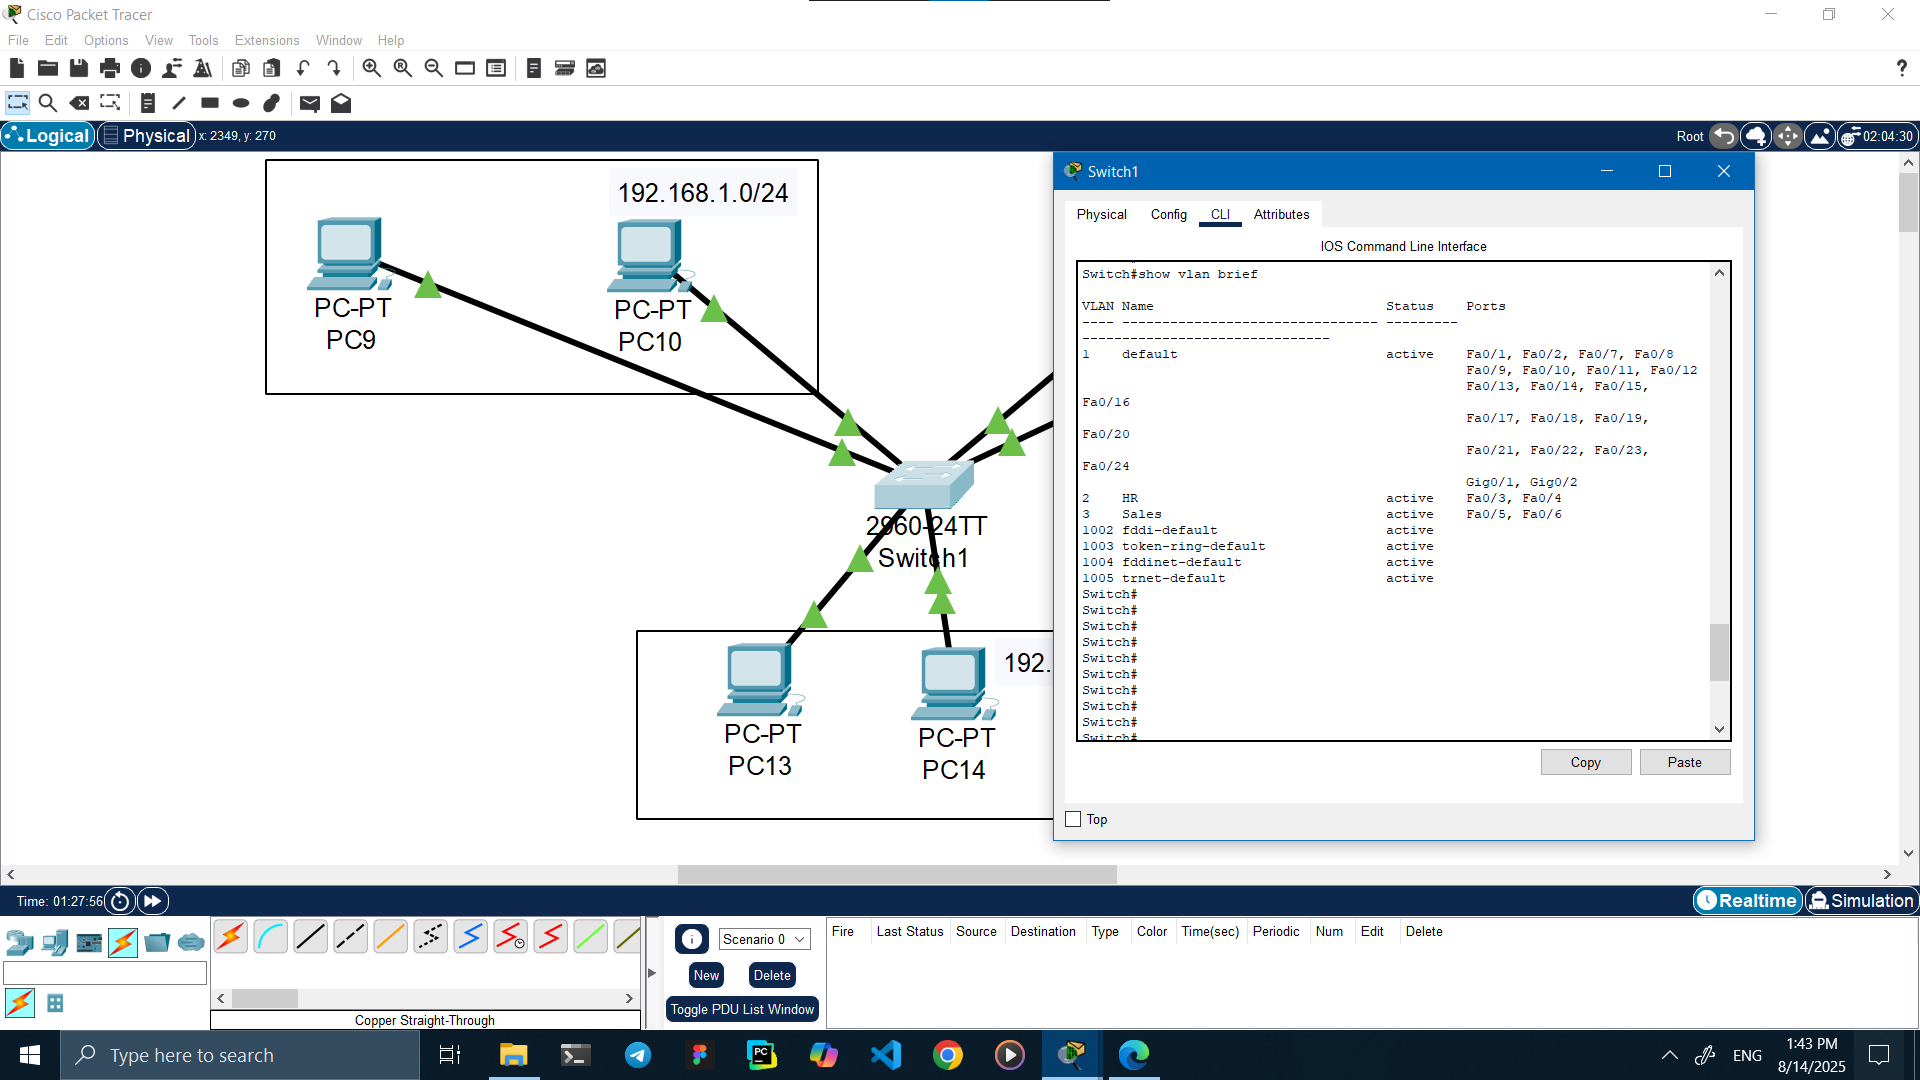
\includegraphics[width=\textwidth]{resources/16.png}
		\caption{اجرای دستور \textenglish{show vlan brief}}
		\label{img:16}
	\end{figure}
	اگر الان در سوییچ دستور \textenglish{show mac address-table} را وارد کنیم، مانند شکل \ref{img:17} نتیجه‌ای ندارد. دلیل این است که هنوز بسته‌ای جا‌به‌جا نشده است. برای حل این مشکل روی یک دستگاه در هر زیرشبکه آن یکی دستگاه را  \textenglish{ping} می‌کنیم تا جدول درست شود.  شکل‌های \ref{img:18} و \ref{img:19} این فرآیند را نشان می‌دهند.
	\begin{figure}[H]
		\centering
		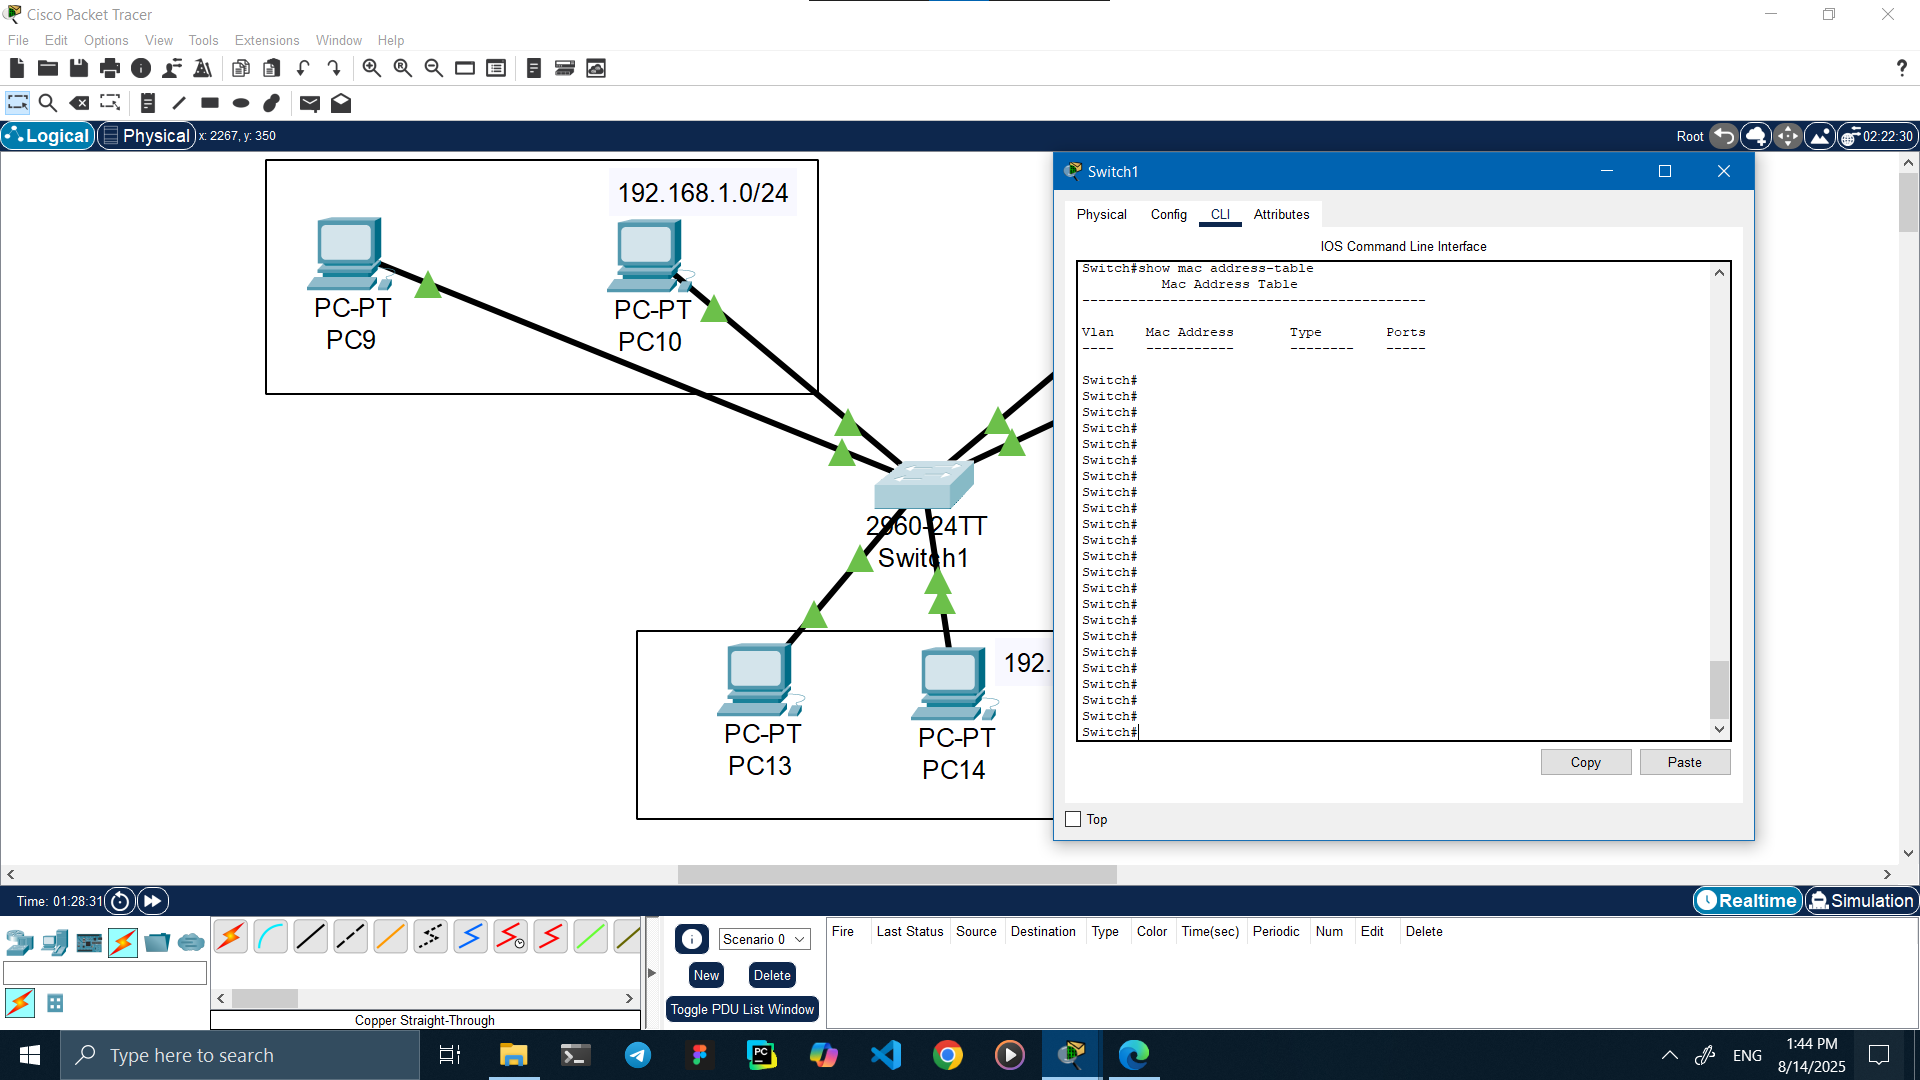
\includegraphics[width=\textwidth]{resources/17.png}
		\caption{اجرای دستور \textenglish{show mac address-table} قبل از \textenglish{ping} کردن}
		\label{img:17}
	\end{figure}
	\begin{figure}[H]
		\centering
		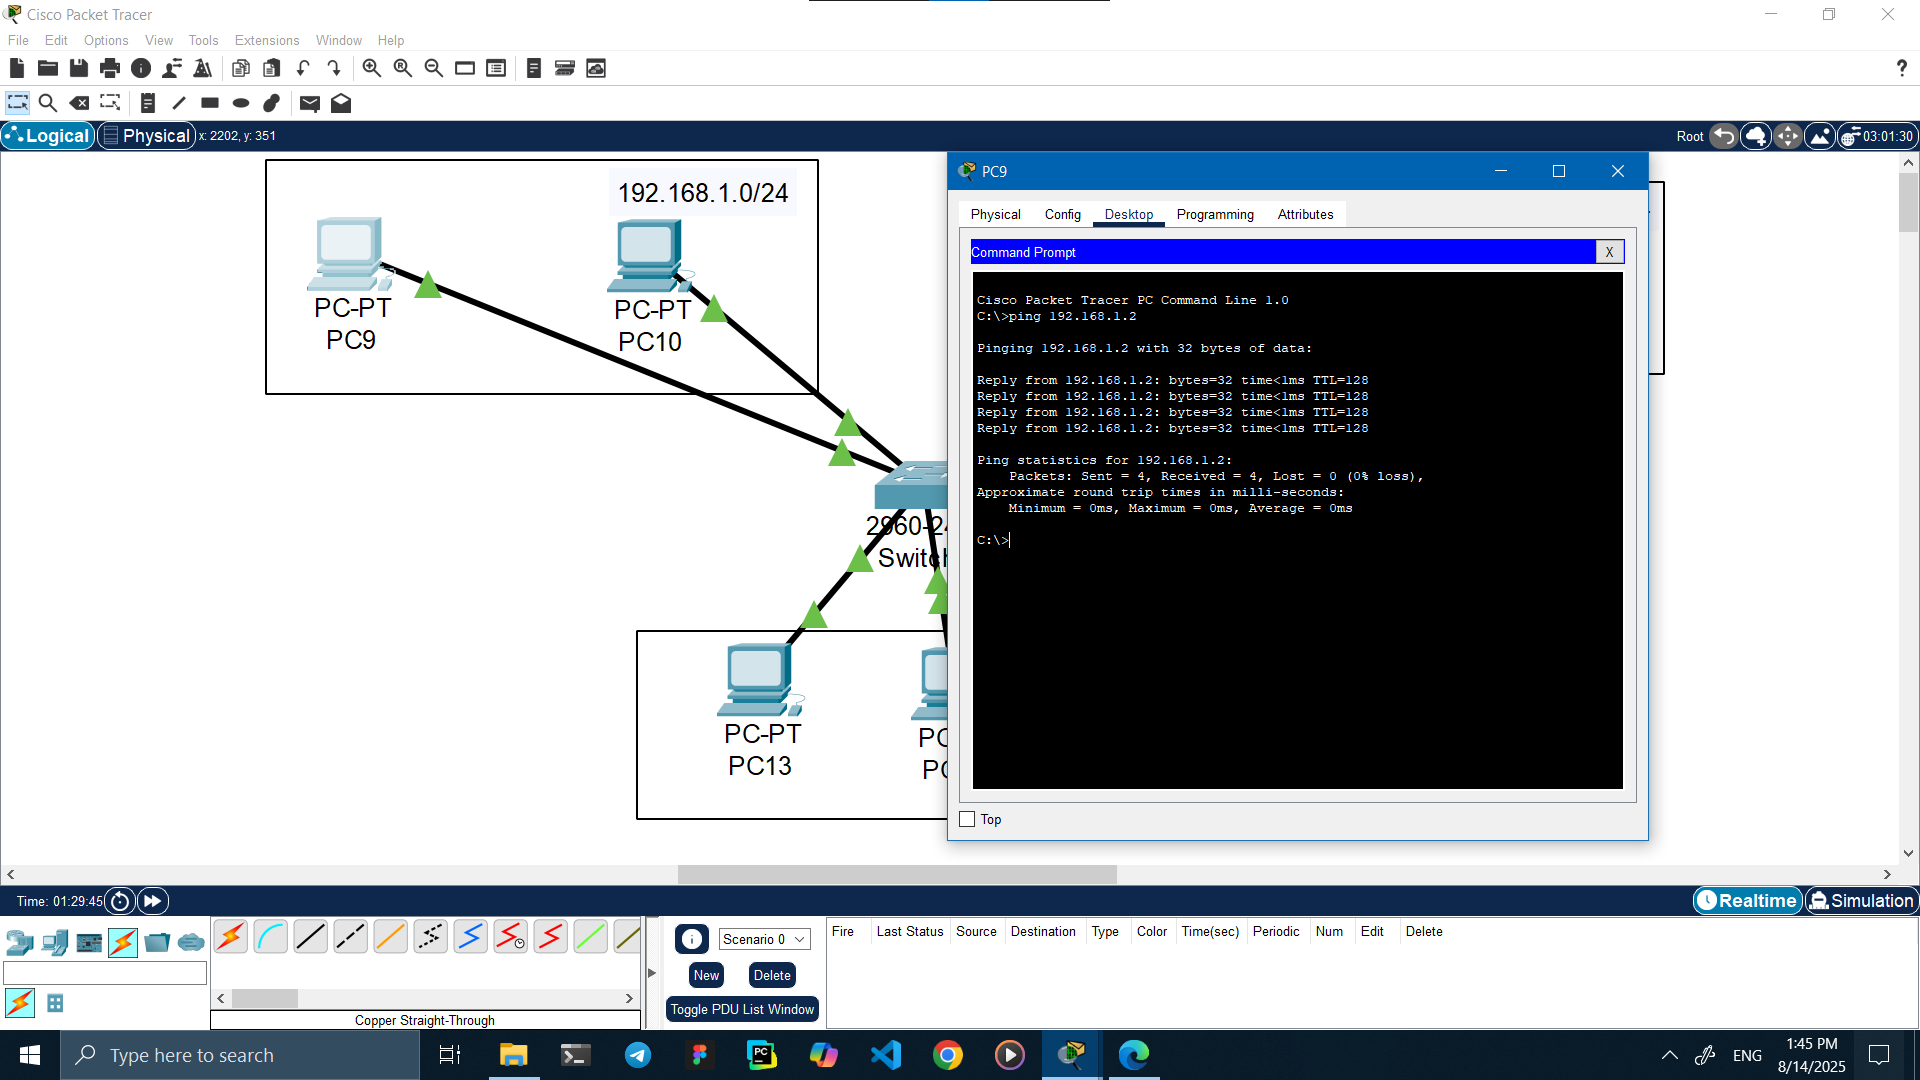
\includegraphics[width=\textwidth]{resources/18.png}
		\caption{اجرای و نتیجهٔ دستور \textenglish{ping} از \textenglish{PC9} به \textenglish{PC10}}
		\label{img:18}
	\end{figure}
	\begin{figure}[H]
		\centering
		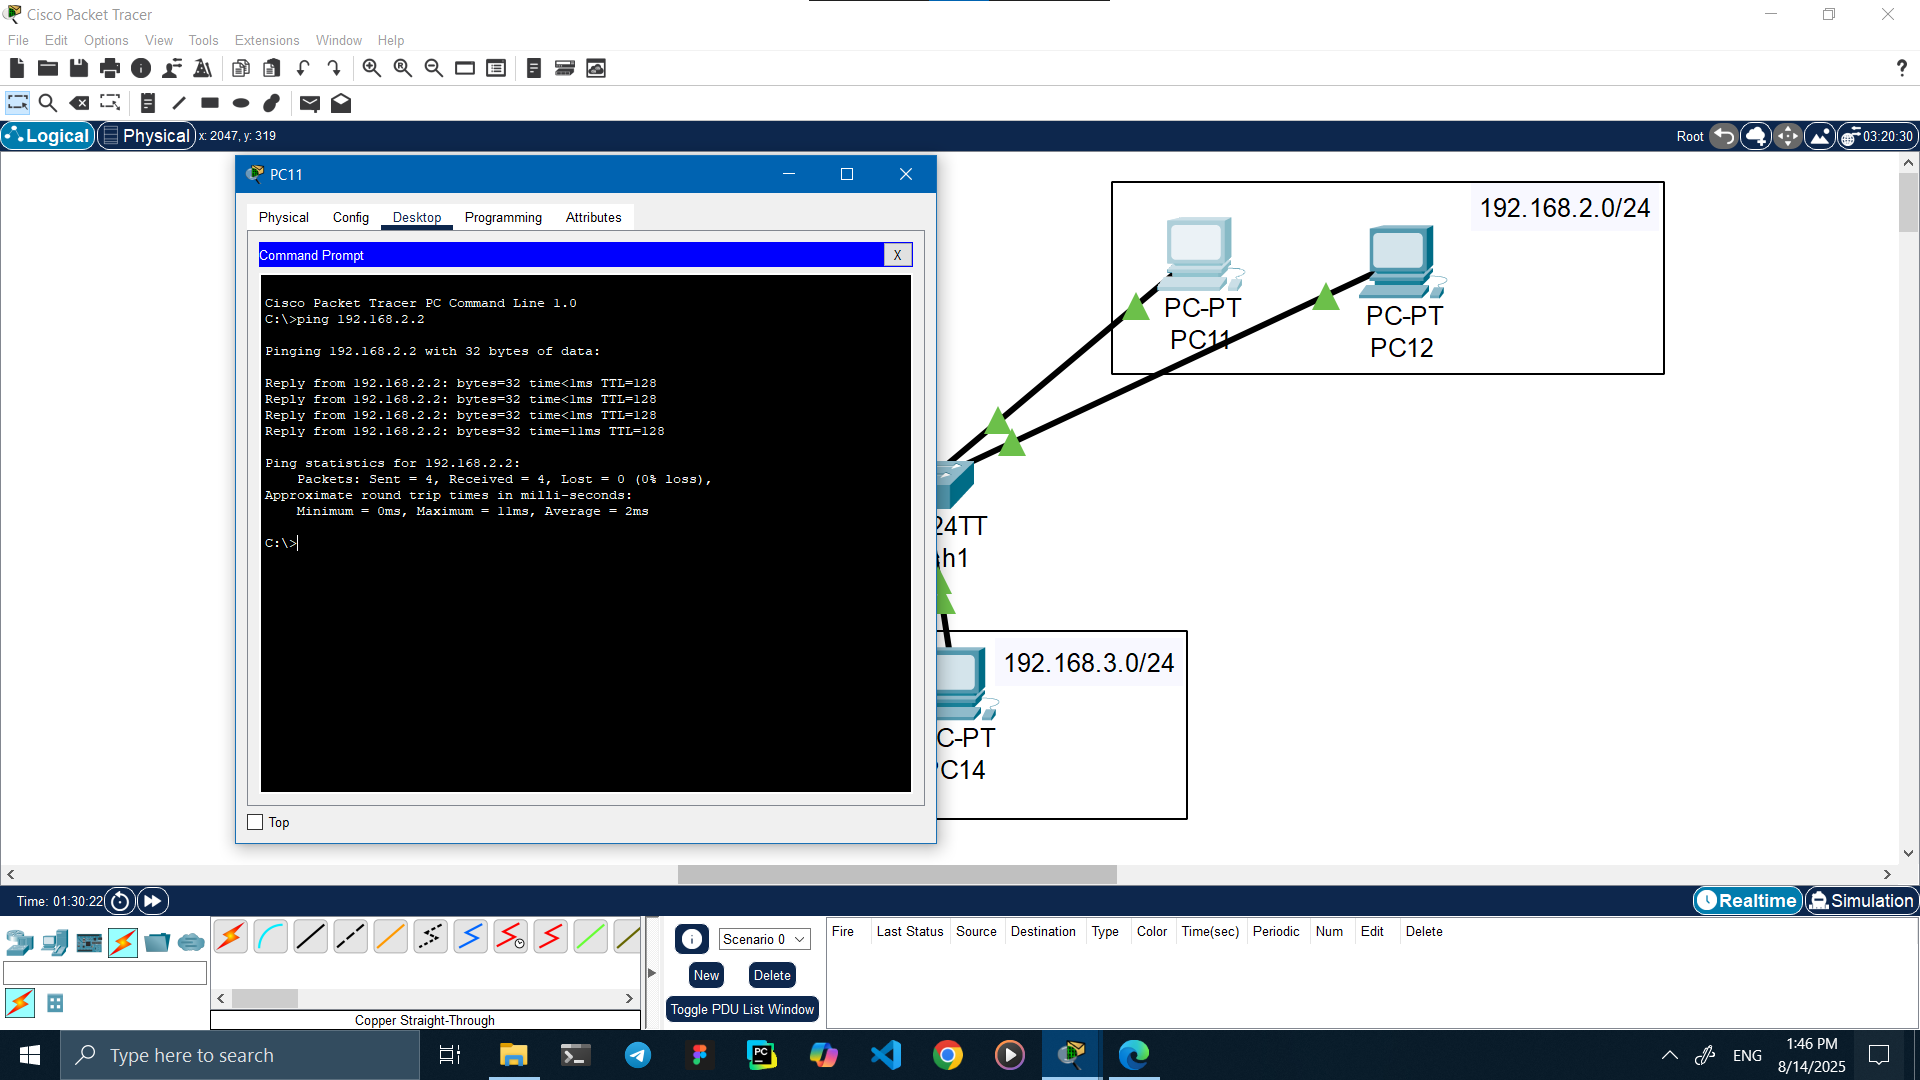
\includegraphics[width=\textwidth]{resources/19.png}
		\caption{اجرای و نتیجهٔ دستور \textenglish{ping} از \textenglish{PC10} به \textenglish{PC11}}
		\label{img:19}
	\end{figure}
	حال اگر دوباره دستور \textenglish{show mac address-table} را اجرا کنیم. حاصل مانند شکل \ref{img:20} خواهد بود و جدول تشکیل شده است. دستور‌های دقیق‌تر مانند
	 \textenglish{show mac  address-table vlan}
	 در نرم‌افزار پشتیبانی نمی‌شود.
	\begin{figure}[H]
		\centering
		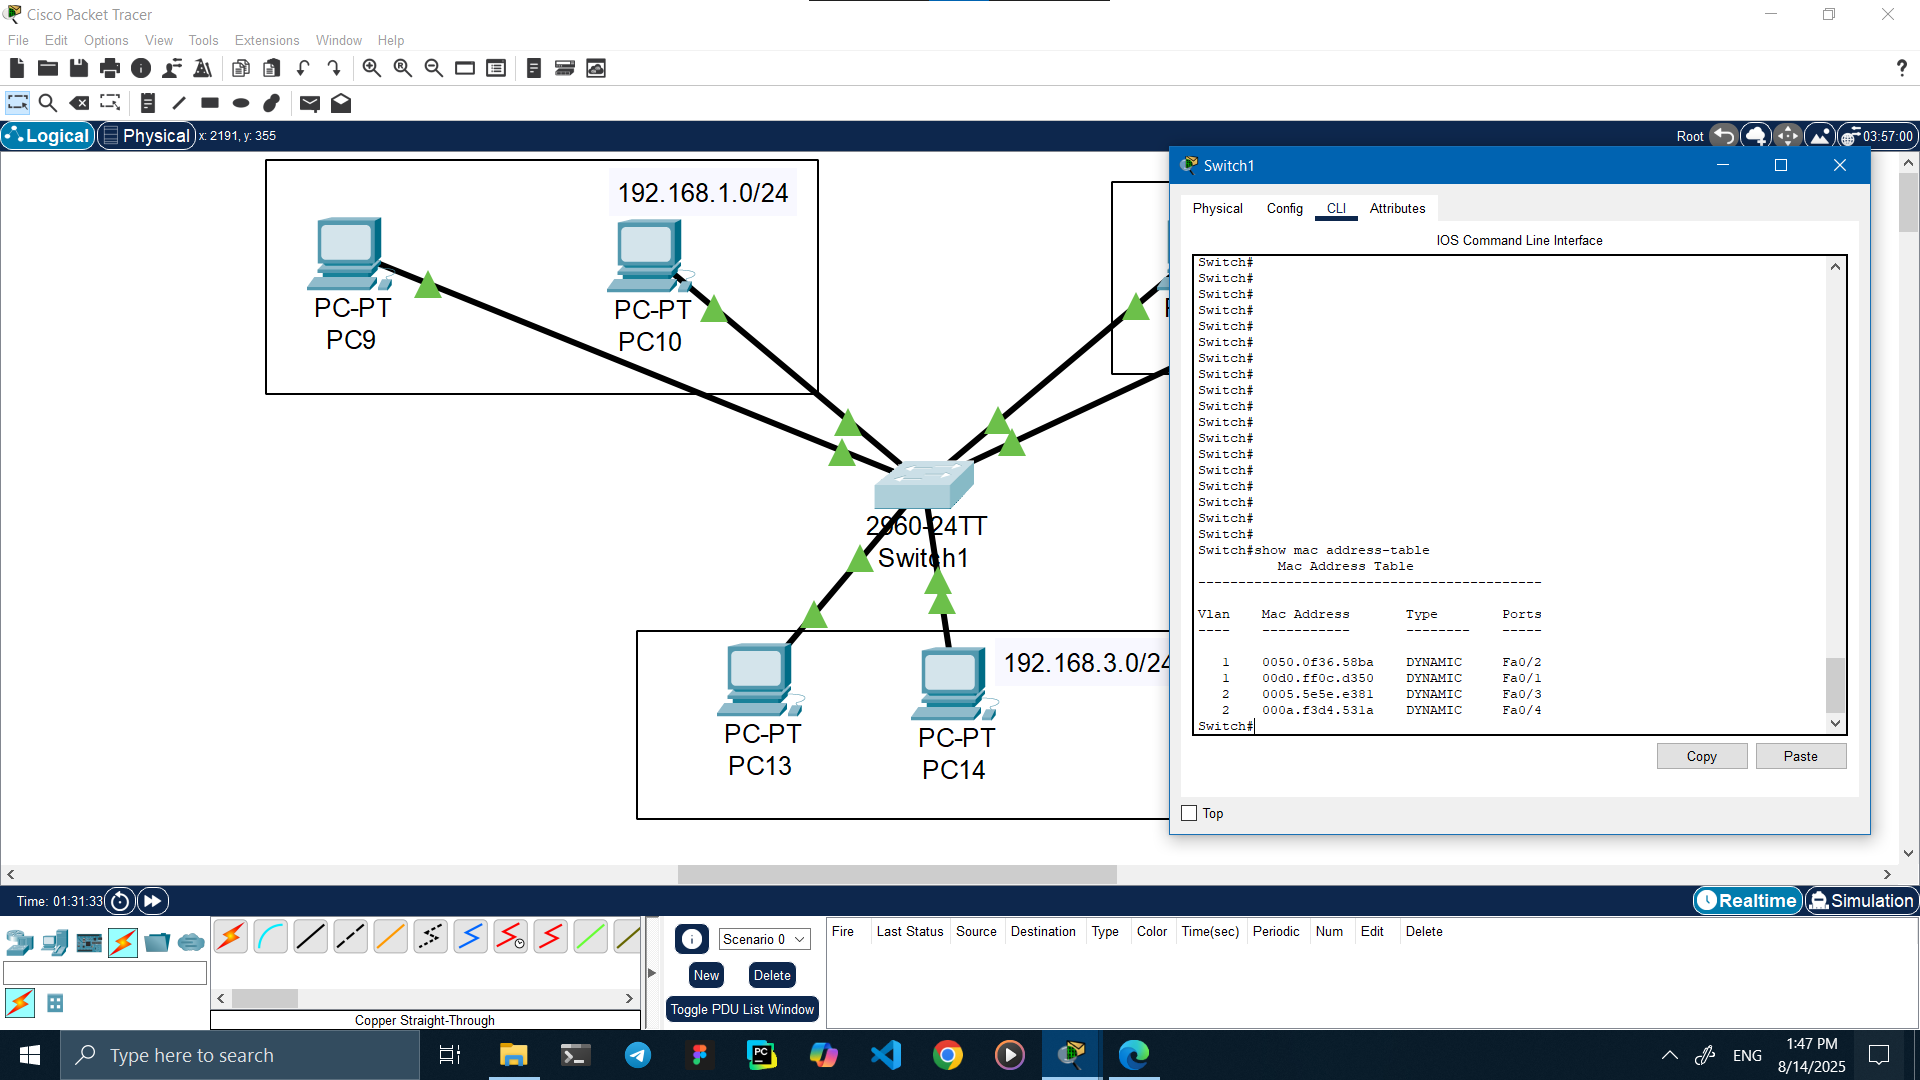
\includegraphics[width=\textwidth]{resources/20.png}
		\caption{اجرای دستور \textenglish{show mac address-table} بعد از \textenglish{ping} کردن}
		\label{img:20}
	\end{figure}
	
	% ==============================
	% References
	% ==============================
	\newpage
	\begin{LTR}
		\printbibliography[title={مراجع}]
	\end{LTR}
	
\end{document}
